%----------------------------------------------------------------------------------------
%	PREÁMBULO
%----------------------------------------------------------------------------------------

\documentclass[10pt, oneside]{book}
\usepackage[paperwidth=17cm, paperheight=22.5cm, bottom=2.5cm, right=2.5cm]{geometry}

%\documentclass[oneside,11pt]{article}


\usepackage{soul}
\usepackage{natbib}
\usepackage{hyperref}
\usepackage{bookmark}
\usepackage{graphicx}             
\graphicspath{{./Figuras/}}
\usepackage[dvipsnames]{xcolor}
\usepackage{todonotes}
\usepackage{makecell}
\usepackage[margin=1in]{geometry}
\usepackage{float}                
\usepackage{amsmath}
\usepackage{amscd}
\usepackage{amsfonts}
\usepackage{amssymb}
\usepackage{bbm}
\usepackage{booktabs}
\usepackage{nameref}
\usepackage{multirow}
\usepackage[nokeyprefix]{refstyle}
\usepackage{rotating}
\usepackage{threeparttable}
\usepackage{afterpage}
\usepackage{lscape}
\usepackage{enumerate}
\usepackage{caption}
\usepackage{subcaption}
\usepackage{epstopdf}
\usepackage{setspace}
\usepackage{svg}
\usepackage{dsfont}
\usepackage{amsthm}
\usepackage{tocloft}
\usepackage{etoc}
\usepackage{lmodern}
\usepackage{bm}
\usepackage[T1]{fontenc}
\usepackage{tgpagella}

\epstopdfDeclareGraphicsRule{.tiff}{png}{.png}{convert #1 \OutputFile}
\AppendGraphicsExtensions{.tiff}

\epstopdfDeclareGraphicsRule{.tif}{png}{.png}{convert #1 \OutputFile}
\AppendGraphicsExtensions{.tif}

\def\sym#1{\ifmmode^{#1}\else\(^{#1}\)\fi}

\usepackage{tikz}
\usetikzlibrary{shapes.geometric, arrows}
\usetikzlibrary{calc}
\usetikzlibrary{matrix}

\tikzset{ 
    table/.style={
        matrix of nodes,
        row sep=-\pgflinewidth,
        column sep=-\pgflinewidth,
        nodes={
            rectangle,
            draw=black,
            align=center
        },
        minimum height=1.5em,
        text depth=0.5ex,
        text height=2ex,
        nodes in empty cells,
%%
        every even row/.style={
            nodes={fill=gray!20}
        },
        column 1/.style={
            nodes={text width=2em,font=\bfseries}
        },
        row 1/.style={
            nodes={
                fill=black,
                text=white,
                font=\bfseries
            }
        }
    }
}


\usepackage{colortbl}
\usepackage{url}
\urlstyle{rm}
\definecolor{darkblue}{rgb}{0,0,.4}
\hypersetup{colorlinks=true, breaklinks=true, citecolor=Maroon, linkcolor=darkblue, menucolor=darkblue, urlcolor=darkblue}

\newtheorem{theorem}{Theorem}
\newtheorem{claim}[theorem]{Claim}
\newtheorem{prop}[theorem]{Proposition} 
\newtheorem{cor}[theorem]{Corollary} 
\newtheorem{assumption}{Assumption} 
\newtheorem{lem}{Lemma} 

\DeclareRobustCommand{\hlgr}[1]{{\sethlcolor{green}\hl{#1}}}


\usepackage{comment}
%para esconder columnas en tablas (enrique)
\usepackage{array}
\newcolumntype{H}{>{\setbox0=\hbox\bgroup}c<{\egroup}@{}}
\linespread{1.25}

\newcommand{\wh}{\widehat}
\usepackage{anyfontsize}

\usepackage[linesnumbered,vlined,ruled,commentsnumbered]{algorithm2e}

\DontPrintSemicolon
\newcommand{\To}{\mbox{\upshape\bfseries to}}
\newcommand{\E}{\mathbb{E}}

\DeclareCaptionFormat{cont}{#1 (cont.)#2#3\par}
%%% HELPER CODE FOR DEALING WITH EXTERNAL REFERENCES
\usepackage{xr}
\makeatletter
\newcommand*{\addFileDependency}[1]{
  \typeout{(#1)}
  \@addtofilelist{#1}
  \IfFileExists{#1}{}{\typeout{No file #1.}}
}
\makeatother


\newcommand*{\myexternaldocument}[1]{
    \externaldocument{#1}
    \addFileDependency{#1.tex}
    \addFileDependency{#1.aux}
}

%\myexternaldocument{OA}

%%%%%%%%%%%%%%%%%%%%%%%%%%%%%%%% DOCUMENT
\begin{document}

%----------------------------------------------------------------------------------------
%	PORTADA
%----------------------------------------------------------------------------------------

\begin{titlepage}
\begin{center}

\title{RPCI}

\textsc{\Large Instituto Tecnológico Autónomo de México}\\[2em]

%Figura
\begin{figure}[h]
\begin{center}

\includegraphics[scale=0.50]{04_Figures/itam_logo.png}
\end{center}
\end{figure}

% Pueden modificar el tamaño del logo cambiando la escala

\textbf{\LARGE El Efecto de la Información en el Cumplimiento del Reporte de Salarios: Evidencia del RPCI del IMSS en México}\\[2em]
%The Impact of Information on Payroll Compliance: Evidence from IMSS's RPCI in Mexico

\textsc{\large Tesis}\\[1em]

\textsc{\large que para obtener el título de}\\[1em]

\textsc{\LARGE Licenciado en Economía}\\[1em]

\textsc{\large Presenta}\\[1em]

\textsc{\LARGE Marco Alejandro Medina Salgado}\\[1em]

\textsc{\large Asesor}\\[1em]

\textsc{\LARGE Dr. Enrique Seira Bejarano}\\[2em]

% Asegúrense de escribir el nombre completo de su asesor

\end{center}

\vspace*{\fill}
\textsc{Ciudad de México \hspace*{\fill} 2023}

\end{titlepage}

%\vspace{.5in}


%\maketitle
%\thispagestyle{empty}
%\begin{abstract}

%Abstract here. 

%\end{abstract}

%\vspace{.3in}

%\textbf{Keywords: }

%\textbf{JEL codes:}

\newpage

\pagenumbering{arabic}
\etocdepthtag.toc{mtchapter}
\etocsettagdepth{mtchapter}{subsection}
\etocsettagdepth{mtappendix}{none}

%----------------------------------------------------------------------------------------
%	DECLARACIÓN
%----------------------------------------------------------------------------------------

\thispagestyle{empty}

\vspace*{\fill}
\begingroup

\noindent
«Con fundamento en los artículos 21 y 27 de la Ley Federal del Derecho de Autor y como titular de los derechos moral y patrimonial de la obra titulada ``\textbf{El Efecto de la Información en el Cumplimiento del Reporte de Salarios: Evidencia del RPCI del IMSS en México}'', otorgo de manera gratuita y permanente al Instituto Tecnológico Autónomo de México y a la Biblioteca Raúl Bailléres Jr., la autorización para que fijen la obra en cualquier medio, incluido el electrónico, y la divulguen entre sus usuarios, profesores, estudiantes o terceras personas, sin que pueda percibir por tal divulgación una contraprestación.»

%The Impact of Information on Payroll Compliance: Evidence from IMSS's RPCI in Mexico

% Asegúrense de cambiar el título de su tesis en el párrafo anterior

\centering 

\vspace{5em}

\rule[1em]{20em}{0.5pt} % Línea para la fecha

\textsc{Fecha}
 
\vspace{8em}

\rule[1em]{20em}{0.5pt} % Línea para la firma

\textsc{Marco Alejandro Medina Salgado}

\endgroup
\vspace*{\fill}

%----------------------------------------------------------------------------------------
%	DEDICATORIA
%----------------------------------------------------------------------------------------

\pagestyle{plain}
\frontmatter

\chapter*{}
\begin{flushright}
\textit{en verdad a qué vengo \\ no lo sé con certeza \\ pero vengo. \\ - Mario Benedetti}
\end{flushright}

%----------------------------------------------------------------------------------------
%	AGRADECIMIENTOS
%----------------------------------------------------------------------------------------

\chapter*{Agradecimientos}

No sé por dónde empezar. Han sido tantos años, tantas horas, tantos sacrificios los que han culminado en este trabajo. Y definitivamente no podría haber llegado hasta aquí sin la ayuda, la guía y el apoyo de tantas personas. \\

\noindent A mis padres. No puedo agradecerles lo suficiente por todo lo que han hecho por mí. Gracias por inculcarme valores tan importantes como el esfuerzo, la perseverancia y la honestidad. Su fuerza, sabiduría, y su apoyo constante han sido la base de todo lo que he logrado. Gracias por confiar siempre en mí. \\

\noindent A mis hermanos, Luis, Armando y Andrea. Gracias por ser mis compañeros, por haberme dado fuerza y ánimo en los momentos más difíciles, por haberme hecho reír tantas y tantas veces. El camino siempre es más ameno con ustedes a lado. Los quiero con todo mi corazón. \\

\noindent A mi asesor, jefe, y coautor, Enrique. Estoy muy agradecido con lo que has hecho por mí. Tu experiencia, tu sabiduría y tu dedicación han sido fundamentales para mi crecimiento académico y personal. Gracias por creer en mí, por enseñarme a pensar críticamente y a hacerme siempre las grandes preguntas. \\

\noindent A mis sinodales, Joyce, Mauricio y Emilio. Por su invaluable orientación y contribución a mi interés en la investigación y desarrollo como investigador. Gracias por enriquecer esta etapa de mi vida y espero seguir contando con su apoyo en mi crecimiento académico y profesional. \\

\noindent A mis amigos economistas, Miguel, Felipe, y Guillermo; a mis amigos matemáticos y actuarios, Carlos, Rubén, Brandon, Santiago y Román; a mis amigos economatemáticos, Fernando y Armando.  Compañeros de trinchera. Gracias por las preguntas, la búsqueda de respuestas y la curiosidad compartida. No podría imaginarme haber cursado la carrera de otra manera que no fuera con ustedes. \\

\noindent A mis amigos, mi segunda familia. Valeria, Camila, Luis, Lina, Mauricio, Sara, Marc, Óscar, Ericka, Sandra, Emilio y Brenda. Ustedes han sido mis compañeros de viaje durante todo este tiempo. Gracias por estar a mi lado, por escucharme, por darme fuerza cuando la necesitaba y por ser mis cómplices en hacer las cosas por la anécdota. Los llevo en mi corazón. \\

\noindent A mis compañeros de trabajo. Emiliano, Esteban, Alondra, Isaac, Max, Roberto, Anna, Erick y Alejandro. Grandes compañeros, mejores personas. Gracias por los sueños y metas compartidas, las curiosidades y las pláticas filosóficas. Estoy seguro que cada uno de ustedes alcanzará todo lo que se propongan. \\

\noindent No hay palabras para expresar la profundidad de mi agradecimiento. Espero que este trabajo sea una pequeña muestra de mi compromiso con la excelencia académica y con el servicio a la sociedad. Y espero que, de alguna manera, pueda retribuir todo lo que me han dado.

%----------------------------------------------------------------------------------------
%	RESUMEN
%----------------------------------------------------------------------------------------

\chapter*{Resumen}

\noindent Las altas tasas de informalidad laboral en países en vías de desarrollo plantean desafíos como la evasión fiscal y distorsiones en la asignación de recursos. Por lo general, la informalidad está asociada con que un trabajador tenga empleo en el sector informal, pero existe un margen intensivo: incluso cuando los trabajadores están inscritos en un empleo formal y tienen beneficios, el salario reportado a las autoridades fiscales puede ser menor que su salario real cuando las empresas tienen la capacidad de elegir los salarios que declaran. Este estudio investiga específicamente el impacto de proporcionar información a los trabajadores sobre el registro y los salarios declarados por su empleador en México, donde podría existir asimetría de información. Centrándose en datos del Instituto Mexicano del Seguro Social (IMSS), el estudio analiza datos administrativos para evaluar los efectos del RPCI (Reporte Personalizado de Cotizaciones en el IMSS) en los salarios registrados de los trabajadores y el registro del empleo ante el IMSS. Utilizando un enfoque de diferencia en diferencias, los resultados revelan que registrarse en el RPCI conlleva un aumento significativo en los salarios reportados (un aumento promedio del 4\% del salario medio un año después), especialmente entre los trabajadores de pequeñas empresas y aquellos que ganan cerca del salario mínimo, en los que observamos un aumento de casi $18\%$ del salario mínimo vigente en 2022. Estos hallazgos mejoran nuestra comprensión de la subdeclaración de salarios y resaltan el impacto potencial de una intervención accesible y altamente efectiva como la provisión de información en el empleo formal en países en desarrollo.

\pagestyle{plain}

\noindent 

%----------------------------------------------------------------------------------------
%	Summary
%----------------------------------------------------------------------------------------

\chapter*{Abstract}

\noindent High rates of labor informality in developing countries present challenges such as tax evasion and distortions in resource allocation. Informality is typically associated with a worker either having a job in the informal sector, but there exists an intensive margin: even when workers are enrolled at a formal job and have benefits, the salary reported to tax authorities may be lower than their true salary when firms have the ability to choose the wages they report. This study specifically investigates the impact of providing workers with information about their employer's registration and reported wages in Mexico, where information asymmetry could exist. Focusing on the Instituto Mexicano del Seguro Social (IMSS) system, the study analyzes administrative records to evaluate the effects of the personalized report, called RPCI (Reporte Personalizado de Cotizaciones en el IMSS), on workers' registered wages and job register to IMSS. Using a difference-in-difference approach, the analysis reveals that registering for the RPCI leads to a significant increase in registered wages (an average increase of 4\% of the mean wage one year later), particularly among workers at small firms and workers earning close to the minimum wage, where we observe an increase of almost $18\%$ of the applicable minimum wage in 2022. This is a huge increase that is difficult to explain if not with possible underreporting from the employer. These findings enhance our understanding of wage underreporting and highlight the potential impact of an accessible and highly effective intervention such as information provision on formal employment in developing countries.

\pagestyle{plain}
\newpage
\noindent 

%----------------------------------------------------------------------------------------
%	TABLA DE CONTENIDOS
%---------------------------------------------------------------------------------------

\tableofcontents

%----------------------------------------------------------------------------------------
%	TESIS
%----------------------------------------------------------------------------------------

\mainmatter % Empieza la numeración de las páginas

\pagestyle{plain}

\chapter{Introduction}

The prevalence of informality in developing countries is a widespread and persistent issue, as highlighted by the International Labour Organization (ILO), which reported that almost 60\% of workers worldwide are engaged in the informal sector \citep{ILO_2018}. In developing countries, the informal sector contributes to nearly a third of the economic activity, which is twice as much as in developed countries.\footnote{\url{https://www.imf.org/external/pubs/ft/fandd/2020/12/pdf/what-is-the-informal-economy-basics.pdf}} In the case of Mexico, the labor informality rate stands at 56.0\% \citep{ENOET120}, with the informal economy accounting for approximately 23\% of the country's GDP \citep{INEGI19}. This significant level of informality carries various consequences, including tax evasion, which undermines the capacity of the state. Moreover, the selective application of taxes to certain workers and not others can lead to distortions in resource allocation and ultimately reduce income \citep{Misallocation}. And in the context of this paper and the intensive margin of informality, lower reported wages lead to lower benefits when they are proportional to the reported wage. \\

The focus of this work is a particular type of labor market informality, namely payroll tax evasion, which manifests along different dimensions. We focus on the understudied margin that pertains to the wage declaration to tax authorities when both the firm and the worker are registered. Social security contributions, income taxes, and payroll taxes create incentives for firms and workers to report lower salaries. The other more commonly studied margins are where firms may choose not to register with the tax authority, or when even if a firm is registered, it might hire workers without reporting them to the social security administration (IMSS), thereby evading taxes and employer contributions. While these two margins are important, as highlighted by \cite{Ulyssea}, public policy that aims to lower informality these two margins could end up harming the compliance in the margin we focus on. Namely, a policy may increase the number of formally registered firms or workers, but lower the proportion of real wages reported to tax authorities. \\

Having firms report employees' wages is no guarantee of accurate reporting in a low-enforcement context like Mexico. Unlike developed countries, where this type of reporting helps mitigate underreporting by workers, the situation is different in developing countries. Registering with IMSS is mandatory by law, and workers have an interest in being registered as it grants them access to free medical services, disability insurance, and contributions to a personal retirement savings account, as we will explain in detail later. However, while disability insurance and the amount deposited in the worker's retirement account increase with the reported wage, access to medical services is not directly tied to the reported wage. More on, most workers didn't check their reported wages until they were about to retire when they needed this information to access their savings or request their pension (less than $5\%$ of workers registered at IMSS do so before they are about to retire), at which point it was difficult to correct any mistakes in the reported wages since former firms they worked may not exist. \\

The situation presents two potential scenarios. On one hand, workers may be misinformed and mistakenly assume that they are formally registered when, in reality, they are not. On the other hand, workers could collude with their employers to determine the reported wage, resulting in reduced taxes and possible shared tax savings. To further explore these matters, we conducted with IMSS a brief survey via email, reaching over 200,000 registered workers. The survey unveiled that only $66.5\%$ of respondents believe their employers report their complete wages to IMSS. In contrast, $10.2\%$ stated that their employers definitely do not report the complete wage, and $23.3\%$ claimed to be uncertain. They also were asked if they had talked with their employer about their reported wage. Interestingly, almost 1 in 5 respondents revealed that they explicitly discussed with their employers which wage should be reported to IMSS. Taken at face value, these findings suggest that a portion of the misreporting may involve collusion, indicating that workers are likely informed about the practice, although the extent may not be substantial. If workers were fully aware, it would be expected that providing them with information about their reported wages would have no impact on their employment status or future reported wages. \\

With this in mind, this paper estimates the causal effect of providing information to workers about whether their employer has registered them with IMSS and the wage that is registered. Using the methodology of \cite{deChaisemartin2022}, we estimate the effect of this information on the worker's registered wage and job termination by exploiting staggered adoption of RPCI (\textit{Reporte Personalizado de Cotizaciones en el IMSS}). The RPCI gives workers a low-cost way to check their formal status in the extensive (being registered) and intensive margin (how many days of work were registered and at which wage level). Before RPCI, workers who wanted to know this information had to schedule an appointment and request it at an IMSS office. Most workers didn't check their reported wages until they were about to retire when they needed this information to access their savings or request their pension, at which point it was difficult to correct any mistakes in the reported wages. \\

Our analysis reveals that, prior to adoption, workers who registered for the RPCI exhibited similar time trends in wages and employment status to those who never registered for the RPCI. However, wages steadily increased precisely when the worker registered for the RPCI, reaching an average increase of 20 pesos one year later (equivalent to approximately 4\% of mean wages). While we observe an increase in the intensive margin, we detect no effect on the extensive margin, i.e., the likelihood of being registered at IMSS. Furthermore, we find that the effect is more pronounced for males, older workers (aged 55 to 65), and those earning 1 to 3 minimum wages. It is also stronger in firms registered in the agriculture and construction sectors, as well as in small firms with fewer than 50 workers. \\

Our study contributes to the existing literature on informality. In their study, \cite{kumler2020enlisting} provide estimations of the median and mean under-reporting of wages in Mexico by comparing cells grouped by characteristics and their reported wages to IMSS against survey responses obtained by INEGI. Their findings reveal a higher prevalence of underreporting among young workers and small firms. Additionally, they investigate the effects of a regulatory reform that aimed to strengthen the connection between reported wages and retirement savings, as well as increase wage transparency for workers. As a result, reported wages to IMSS saw an increase, particularly among the younger cohorts who were most impacted by the reform. However, due to the reform's simultaneous changes in benefits and information provided to workers regarding reported wages, it becomes challenging to disentangle the specific influence of wage transparency versus incentives to report wages as the primary driving force behind the observed outcomes.\footnote{It is worth noting that the treatment-control comparisons involve comparing older and younger workers, which introduces the possibility of differential time trends due to the reform coinciding with the tequila crisis, a period of macroeconomic instability.} \\

\cite{kumler2020enlisting} also acknowledge that the "extent to which workers are aware of underreporting by their employers and, consequently, the extent to which the observed effects of the pension reform are due to changes in incentives versus information changes" remain open questions. We complement this by being able to separate the effect of information from changes in benefits. More on, our results use panel data which can identify individuals and their changes, instead of relying on estimating the difference between cells created by worker characteristics. More on, as highlighted by \cite{Ulyssea}, policies that seek to lower informality in a specific margin could trigger an increase in another margin. Specifically, we analyze how the reported wages increased while the probability of being registered remained unchanged. \\

\chapter{Context} \label{context}

\section{Background of the Instituto Mexicano del Seguro Social (IMSS)}

The Instituto Mexicano del Seguro Social (IMSS) is the Mexican social security agency. It plays a crucial role in providing medical services and managing retirement resources for formally employed individuals in the country. IMSS benefits encompass several areas, including occupational risk insurance, maternity insurance, disability schemes, and pensions, among others. There exists more than one scheme offered by IMSS. According to the Social Security Law, individuals can be affiliated with the IMSS under either the Mandatory or Voluntary scheme, each with its own set of benefits, eligibility criteria, and financing methods. This research primarily focuses on job registrations within the IMSS, which primarily consist of workers who are affiliated through their employers under the Mandatory Scheme. However, it should be acknowledged that the Voluntary Scheme may also include self-employed individuals and independent employers, which would be part of our sample. \\

The Mandatory Scheme requires individuals to be affiliated with the IMSS through their employers, as a result of their subordinated and paid employment relationship, making insurance coverage obligatory. As of December 2021, this category represented 69.6\% of the insured population \citep{IMSS22}. Notably, Modality 10 (Permanent and Temporary Workers in urban areas) holds the highest affiliation rate within this scheme, comprising 96.6\% of the employed population in the Mandatory Scheme affiliated as of December 2021 (19,439,594 insured workers). \\

The Voluntary Scheme results from an individual or collective decision. This includes individuals enrolled in the Family Health Insurance (SSFAM) and the Voluntary Insurance for Students, among others. As of December 2021, this group constituted the remaining 30.4\% of insurance coverage under IMSS. The predominant category within the Voluntary Scheme was the Voluntary Health Insurance for Students, accounting for 89.2\% of the total. Other categories within the Voluntary Scheme, such as Family Health Insurance (Modality 33), Voluntary Continuation (Modality 40), and insurance for public servants at the federal, state, and municipal levels (Modalities 36, 38, and 42), covered 10.2\% of the total. The lowest rates of affiliation were observed among individual employers, domestic workers, self-employed individuals, and voluntary enrollment of agricultural workers, collectively representing 0.5\% of the voluntary coverage until December 2021. \\

According to the Social Security Law, the benefit scheme of the Mandatory Scheme comprises all the insurance coverage offered by the IMSS:

\begin{itemize}
    \item Work-related Risks (WRR).
    \item Sickness and Maternity (SAM).
    \item Disability and Life (DL).
    \item Retirement, Old Age, and Elderly Unemployment (ROAEU).
    \item Daycare Centers and Social Benefits (DCSB). 
\end{itemize}

Although many of these benefits and insurance coverage provide fixed or in-kind benefits, some of them also incorporate elements that depend on the reported wage. However, there are two exceptions: Daycare Centers and Social Benefits, which are not tied to the reported wage. \\

The Work-related Risks Insurance offers a temporary incapacity subsidy equivalent to 100\% of the wage registered at IMSS at the beginning of the incapacity. This subsidy is provided for a period of up to 52 weeks, as determined by the medical services of IMSS. \\

Under the Sickness and Maternity coverage, a subsidy equivalent to 60\% of the last reported wage is granted starting from the fourth day of incapacity and continues for up to 52 weeks. Maternity coverage, on the other hand, provides a subsidy equivalent to 100\% of the last reported wage for 42 days before and after childbirth. \\

In the case of Disability and Life coverage, a worker is considered disabled when they are unable to earn more than 50\% of their usual earnings due to a non-work-related accident or illness. \\

Lastly, the Retirement, Old Age, and Elderly Unemployment Benefits are dependent on the reported wage and are linked to the individual's savings or pension. \\

Under the Mandatory Scheme, employers are responsible for reporting the job status of workers to the IMSS, including information such as wages earned and days worked. The taxes and social security contributions paid by employers are proportionate to the reported wage. However, it has been observed that some employers may underreport the actual wages earned by their workers \citep{kumler2020enlisting}. This practice can have negative consequences for workers since social security, retirement, and pension benefits are also tied to the reported wage. \\


\section{Motivation}

We conducted an online survey of workers enrolled at IMSS in August 2021. The survey was sent via email to a random sample of workers. Figure \ref{fig:hist_knowledge_register_survey} shows the answers to some of the survey questions, related to knowledge about IMSS and wage reporting to the IMSS. This survey serves as motivation for this paper. \\

\begin{figure}[H]
    \centering
    \caption{Knowledge about IMSS and worker's reported wages \label{fig:hist_knowledge_register_survey}}
    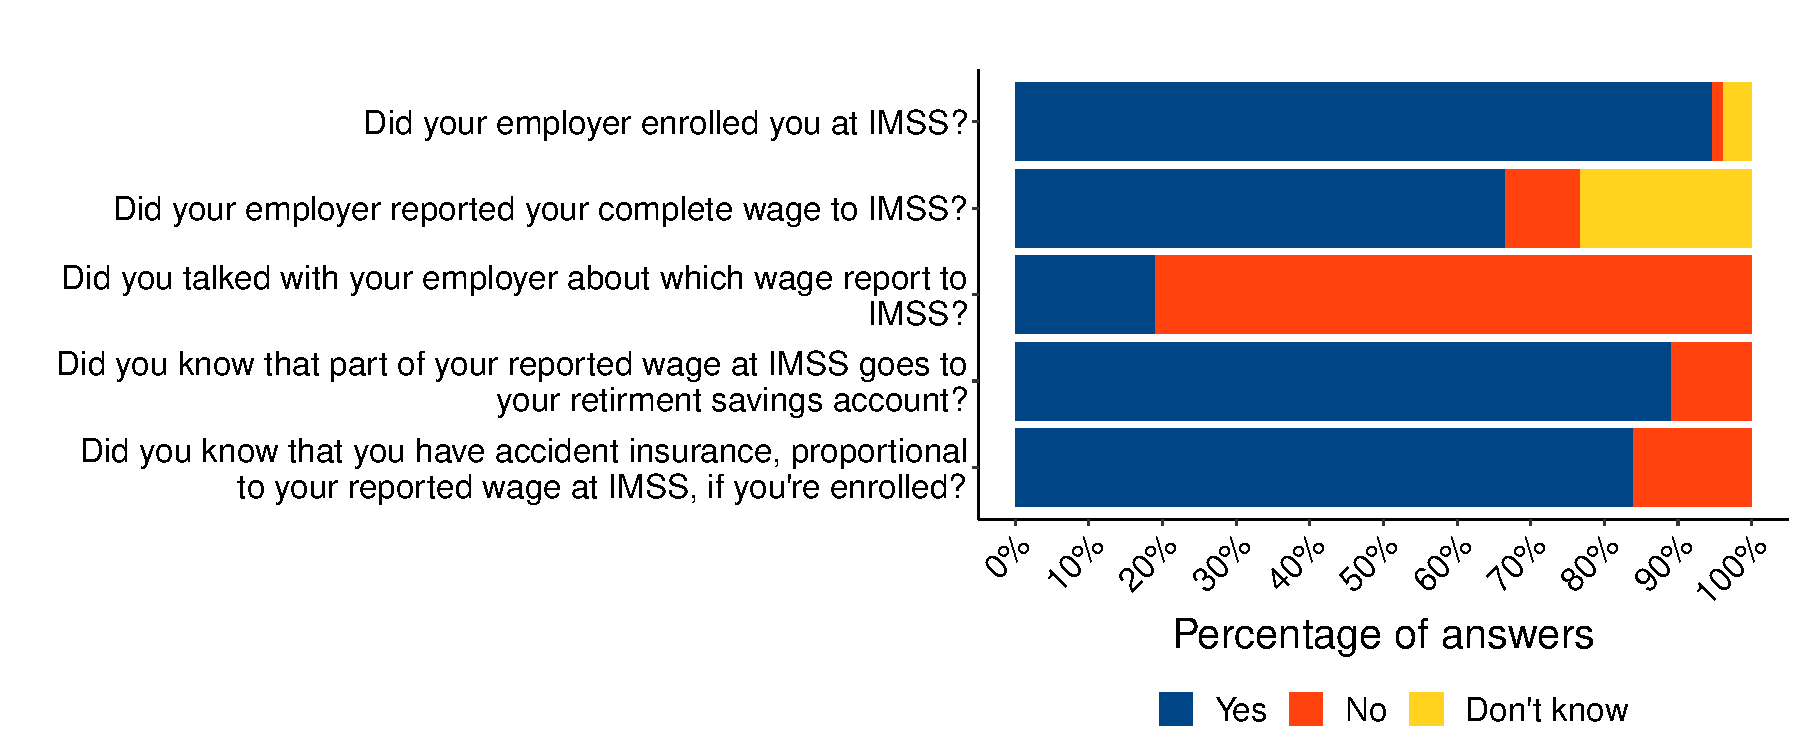
\includegraphics[width=\textwidth]{04_Figures/worker_survey/hist_knowledge_register_survey.pdf}
\end{figure}
\scriptsize{\textit{Notes}: This figure shows answers to questions about IMSS and wage reporting from the worker survey. \textit{Sample:} 233,709 answers from a survey conducted via email to workers enrolled at IMSS during August 2021. Questions 1-2, about the worker's employer, included the option "I don't know". Questions 3-5 ask about the worker's actions or knowledge and didn't include the option "I don't know".
} \\

\normalsize

We find that not all workers know the status of their enrollment in the IMSS. Even though all workers were actually enrolled at IMSS, $1.5\%$ of workers said they weren't enrolled, and $4\%$ said they didn't know if they were enrolled. Moreover, workers don't always know their reported wages or know the existence of wage underreporting by their employer. When we asked in the survey if their employer reported their complete wage to the IMSS, $23.3\%$ answered that they didn't know, and $10.2\%$ said no. Most workers don't talk with their employers about which wage will be reported to the IMSS. $81\%$ of workers say they didn't talk with their employer about which wage to report to the IMSS. On the other hand, workers are aware that their benefits depend on the reported salary. $88.9\%$ report being aware that part of their reported wage goes to their savings accounts. $83.7\%$ report being aware of the existence of accident insurance when being enrolled at IMSS, which is proportional to their reported wage. \\

Wage underreporting happens to different extents, and some workers are aware of its occurrence. Workers could agree to underreport their wages if the gains of paying fewer taxes are given to them and are more valued than the benefits obtained at the IMSS. If underreporting was part of an agreement, receiving information about the worker's current job would not affect her since she already knows this information. The survey answers don't exactly reflect this story. Most workers don't talk with their employers about their wages, and many don't know if their complete wage is reported. With this in mind, if underreporting happened, receiving information about their current job enrollment could trigger workers to force higher compliance in wage reporting from their employers.



\section{The RPCI Initiative}

Workers often only become aware of wage underreporting when they are nearing retirement and request the consolidated statement of the contributions made in their name from the IMSS. This statement contains detailed information about each job the worker has been registered for at the IMSS, including wages, the name of the employing firm, and tenure. By the time workers discover underreporting, there is little they can do to rectify the situation, since firms may no longer exist, and providing evidence of the correct former wages can be difficult. Only about $5\%$ of workers request this statement prior to their retirement age, and most of them only see it once they are about to retire. \\ 

To address this issue, the IMSS has implemented the RPCI (Reporte Personalizado de Cotizaciones en el IMSS) initiative. The RPCI provides workers with easy access to information about their job registration, including their current reported wage and the legal name of their employer. Workers can register for the RPCI through the IMSS app and receive their personalized reports on a monthly basis after registration. \\

Figure \ref{rpci_example} illustrates a screenshot of the IMSS app and provides an example of the PDF report that workers receive through the RPCI. The objective of this initiative is to enhance workers' access to information regarding their job registration and to promote compliance through worker enforcement.\footnote{Figure \ref{rpci_flyers} shows flyers announcing the RPCI app. Figure \ref{rpci_register} shows how the workers register for the RPCI within the IMSS app.} \\ 

\begin{figure}[H]
    \caption{RPCI example}
    \label{rpci_example}
    \begin{center}
    
    \begin{subfigure}{0.49\textwidth}
    \caption{RPCI within the IMSS Digital app}
    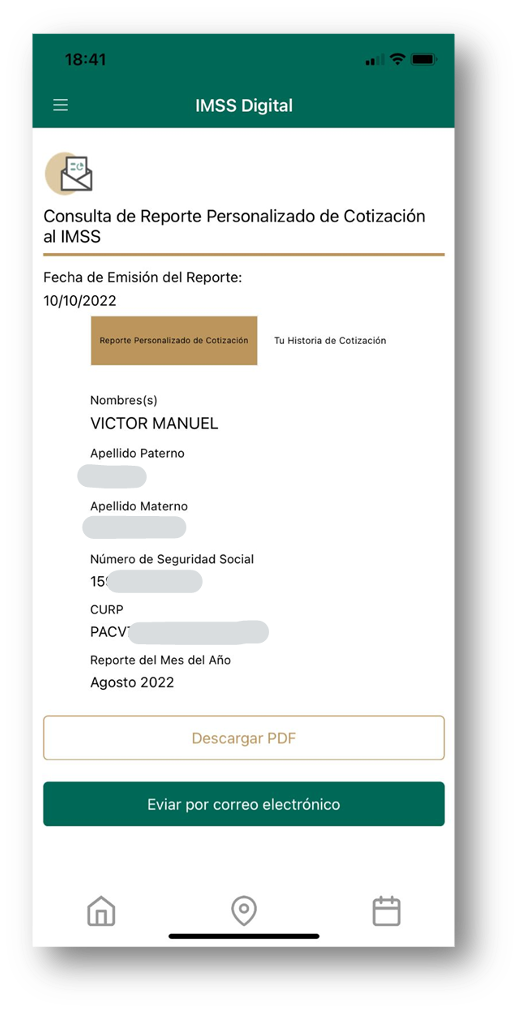
\includegraphics[width=\textwidth]{04_Figures/rpci_app/rpci_2.png}
    \end{subfigure}
    \begin{subfigure}{0.49\textwidth}
    \caption{RPCI PDF file}
    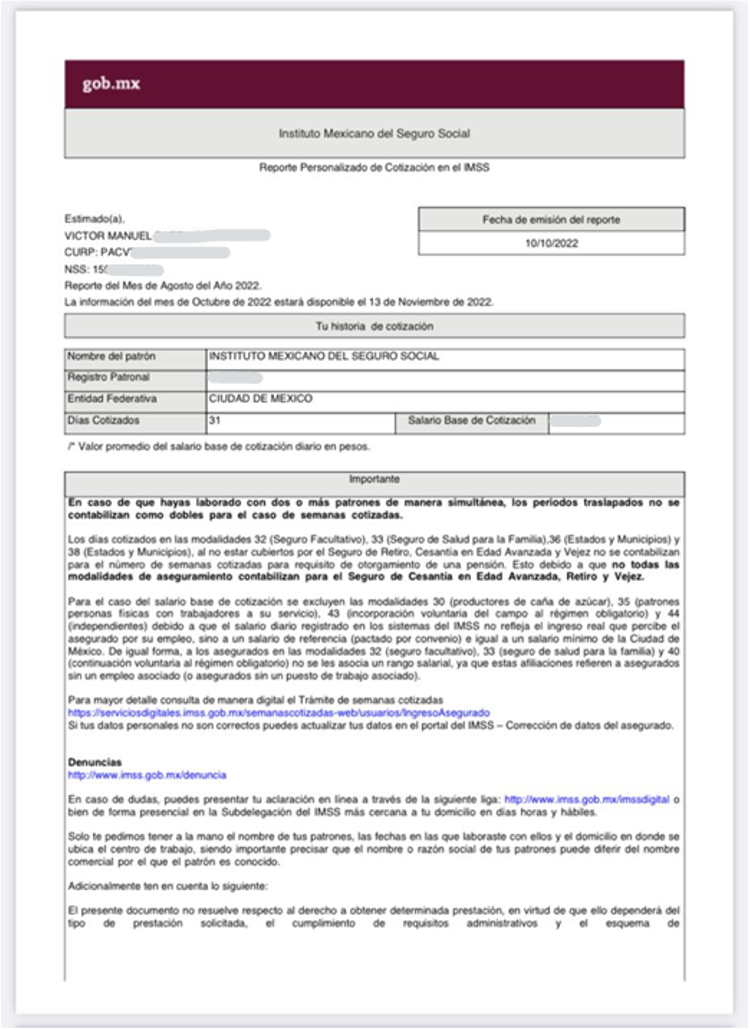
\includegraphics[width=\textwidth]{04_Figures/rpci_app/rpci_3.png}
    \end{subfigure}
    

    \end{center}
\end{figure}
\scriptsize{
\noindent Figure (a) shows the IMSS Digital app, where once the worker is registered for the RPCI, the worker can download their report in PDF or receive it via email. Figure (b) shows an example of the PDF for the RPCI. The report includes the worker's job registered information, such as wage and the firm the worker is registered at.
} \\

\normalsize



\chapter{Data} \label{data}

For our main analysis, we use administrative data on workers' records from IMSS. We use a monthly panel dataset for a random sample of workers registered at IMSS during January 2021, one month before the RPCI launch. The dataset follows the workers from January 2018 to February 2022. It includes variables on the workers' registration, such as their wage, industry, age group, firm, job modality, and state. It also contains a variable on when the worker registers for the RPCI. We will refer to this dataset as the worker panel data. \\ 

Table \ref{tab:summary_stats_rpci} shows summary statistics for this data. We observe more than $1,400,000$ workers and $339,000$ firms. Our sample was a random sample of workers enrolled at the Mexican Institute of Social Security (IMSS) during 2020 and January $2021$, before the RPCI launch. Around $2\%$ of the workers in the sample registered for the RPCI at some point in our data. Workers in our sample were registered at IMSS $96\%$ of time in our data. $39\%$ of them were women, $21\%$ were in an outsourcing schedule and $10\%$ were eventual workers. The average daily wage registered in our sample is $\$492.44$ (MXN)\footnote{Approximately $\$25$ (USD) at the time the RPCI was launched, February 2021.}. \\

\begin{table}[H]
\footnotesize
\centering
\begin{threeparttable}
\centering
\caption{Summary Statistics\label{tab:summary_stats_rpci}}
%\textit{Do file: summary_stats_rpci.do}

\begin{tabular}[t]{@{}l}
\toprule
\toprule
\begin{tabular}[t]{lccc}
\input 03_Tables/muestra_10porciento/summary_stats_rpci
\midrule
Workers & & & 1,412,210\\
Firms & & & 339,884\\
\end{tabular}

\tabularnewline 
\bottomrule
\bottomrule

\end{tabular}

\begin{tablenotes}
\setlength\labelsep{0pt}
\scriptsize
\item \textit{Notes}: This table shows summary statistics on selected variables for our final sample. \textit{Sample:} Panel data for a random sample of the workers enrolled at the Mexican Institute of Social Security (IMSS) during 2020 and January 2021 (before the RPCI launch). \textit{Registered for RPCI} is a dummy where 1 means worker $i$ registered for the RPCI at some point in our sample. \textit{Enrolled} is a dummy variable where 1 means worker $i$ was enrolled at IMSS during period $t$. \textit{Women}, \textit{Outsourcing}, and \textit{Eventual} are dummies where 1 means worker $i$ is a woman, an outsourced worker, or an eventual worker, respectively. \textit{Wage} is registered wage for worker $i$ during period $t$. \textit{N} is the number of non-missing observations for each variable. Wage and worker characteristics are only available if the worker was registered during period $t$. \textit{Workers} and \textit{Firms} are the number of unique workers and firms in our sample. %This table is referenced in \hyperref[subsec:workers]{Section} \ref{subsec:workers}.
\end{tablenotes}
\end{threeparttable}
\end{table}


Workers have registered for the RPCI since it was launched in February 2021. Figure \ref{hist_download} shows the number of registers per month since the RPCI was launched. Each download month is considered a cohort in terms of the analysis in this work. Once workers register for the RPCI, they receive the report each month, in the IMSS app or via email. This creates a staggered design we can exploit. More on, not all workers registered at IMSS have registered for the RPCI, which means there exists a pure control group to compare each treatment cohort to.  \\

\begin{figure}[H]
    \caption{RPCI registers by month}
    \label{hist_download}
    \begin{center}
    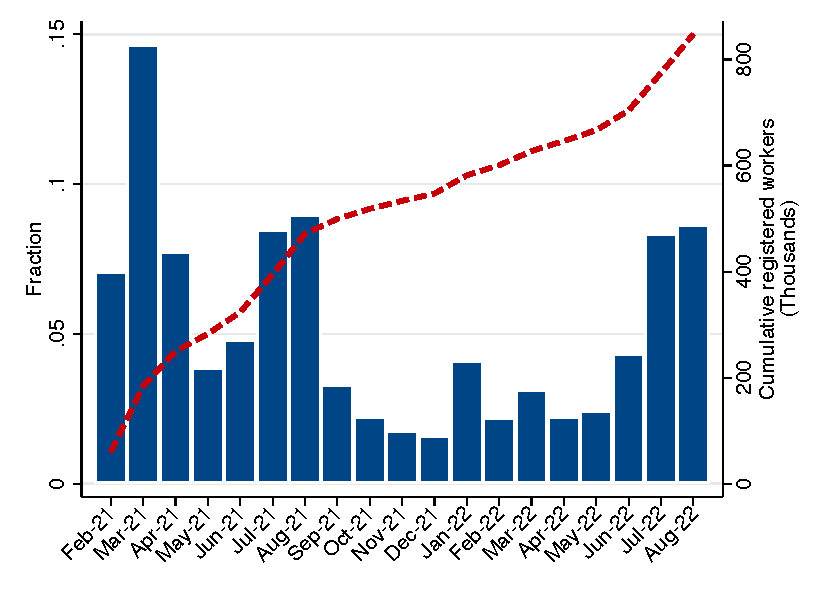
\includegraphics[width=0.65\textwidth]{04_Figures/muestra_1porciento/hist_download_month.pdf}
    \end{center}
\end{figure}
\scriptsize{
\noindent This figure shows the total number of workers registered for the RPCI. The right y-axis measures the fraction of workers who registered for the RPCI during each month from the total workers who registered for the RPCI. The left y-axis measures the cumulative number of workers who registered for the RPCI.
} \\

\normalsize

Apart from the administrative data, we have data obtained through a survey we conducted via email with IMSS. The survey received 233,709 responses from workers who answered the survey. The survey included questions on the wage the worker earns and the wage the worker thinks is registered at IMSS. It also includes questions to test the worker's level of knowledge about IMSS. This allows us to investigate the level of knowledge workers have about their reported wages. We will refer to this dataset as the survey data. This is the data where the information for Figure \ref{fig:hist_knowledge_register_survey} comes from.


\chapter{Specification} \label{specification}

Our main analysis is conducted using panel data. The treatment in our context is registration for the RPCI, which follows a staggered treatment design. Workers have the option to register for the RPCI at any time after its launch, and they can access their personalized reports every month following registration. Consequently, we observe treatment cohorts for each month since the launch of RPCI. Moreover, not all workers registered at IMSS have enrolled in the RPCI, creating a pure control group for comparison with each treatment cohort when using causal inference methods. \\

To evaluate the causal treatment effect of registering for the RPCI, we employ a difference-in-difference (DID) analysis. Initially, we utilize a simple two-way fixed effects (TWFE) specification. However, recent literature (\citealt{de2020two}; \citealt{callaway2021difference}; \citealt{sun2021estimating}) has highlighted that TWFE estimates can be misleading or biased due to the weighted average of average treatment effects (ATEs) when negative weights or non-rare forbidden comparisons are involved, especially in cases with heterogeneous treatment effects across different treatment cohorts over time. Several authors have proposed alternative specifications to address this issue. Consequently, we also employ the specification proposed by \cite{de2020two}\footnote{The estimators proposed by \cite{callaway2021difference} and \cite{sun2021estimating} are computationally challenging to implement with large samples like ours, as they involve calculating 2x2 differences between individuals and periods. \cite{de2020two} can be optimized to handle large samples, which is why we selected this estimator from among those proposed by the recent literature.}, incorporating the robust dynamic option to account for potential heterogeneous treatment effects across cohorts. \\

\section{Difference-in-Differences}

With two groups and two periods, a difference in differences (DID) estimator compares the outcome evolution from period 1 to 2 between a treatment group $T$ that switches from untreated to treated, and a control group $C$ that is untreated at both dates: \\

$$\text{DID} = Y_{T,2} - Y_{T,1} - (Y_{C,2} - Y_{C,1})$$

DID relies on a parallel trends assumption. In the absence of the treatment, both groups would have experienced the same outcome evolution. Specifically, for every group $g \in \{T, C\}$ and period $t \in \{1, 2\}$, let $Y_{g,t(0)}$ and $Y_{g,t(1)}$ denote the potential outcomes in group $g$ at period $t$ without and with the treatment, respectively. Parallel trends require that the expected evolution of the untreated outcome be the same in both groups. \\

\textbf{Assumption: Parallel Trends.} The expected evolution of the untreated outcome is the same in both groups: 

$$ \mathbb{E}[Y_{T,2(0)} - Y_{T,1(0)}] = \mathbb{E}[Y_{C,2(0)} - Y_{C,1(0)}]$$

Under that assumption, DID is unbiased for the average treatment effect (ATE) for the treated group at period 2 \citep{abadie2005semiparametric}:  

\begin{equation}
\begin{aligned}
\mathbb{E}[\text{DID}] &= \mathbb{E}[Y_{T,2} - Y_{T,1} - (Y_{C,2} - Y_{C,1})] \\
&= \mathbb{E}[Y_{T,2}(1) - Y_{T,1}(0) - (Y_{C,2}(0) - Y_{C,1}(0))] \\
&= \mathbb{E}[Y_{T,2}(1) - Y_{T,2}(0)] + \mathbb{E}[Y_{T,2}(0) - Y_{T,1}(0)] - \mathbb{E}[Y_{C,2}(0) - Y_{C,1}(0)] \\
&= \mathbb{E}[Y_{T,2}(1) - Y_{T,2}(0)]
\end{aligned}
\end{equation}

where the last equality follows from the parallel trends assumption. Parallel trends assumption is partly testable, by comparing the outcome trends of groups $T$ and $C$ before group $T$ received the treatment. In practice, such pre-trend tests sometimes fail, but other times they indicate that the two groups were indeed on parallel paths before $T$ got treated. \\

Motivated by the fact that in the two-groups and two-periods design described above, DID is equal to the treatment coefficient in a two-way fixed effects (TWFE) regression with group and period fixed effects, researchers have also estimated TWFE regressions in more complicated designs with many groups and periods, variation in treatment timing, treatments switching on and off, and/or non-binary treatments. Recent research has shown that in those more complicated designs, TWFE estimators are unbiased for an ATE if parallel trends hold, and if another assumption is satisfied: the treatment effect should be constant, between groups and over time. Unlike parallel trends, this assumption is unlikely to hold, even approximately, in most of the applications where TWFE regressions have been used. \\

In practice, the TWFE idea is implemented by regressing $Y_{g,t}$, the outcome in group $g$ and at period $t$, on group fixed effects, period fixed effects, and $D_{g,t}$, the treatment of group $g$ at period $t$. Such two-way fixed effects regressions are probably the most commonly used technique in economics to measure the effect of a treatment on an outcome. Researchers have long thought that TWFE estimators are equivalent to differences-in-differences (DID) estimators, but recent research has shown it isn't \citep{DID_survey}. The main problem relies on the existence of possible negative weights that make the estimator a non-convex combination of effects, that arise from possible forbidden comparisons between treatment and control groups. \\

\section{Alternative estimators}

With a binary treatment, de Chaisemartin and D'Haultfœuille (2020) propose using the Difference-in-Differences estimator DIDM to identify the Average Treatment Effect on the Treated (ATT) in a research design. This estimator provides a weighted average of two types of DIDs across time periods. \\

To define the estimator, let us consider a potential outcomes framework as introduced by \cite{rubin1974estimating} and follow the notation used in \cite{de2020two}. We denote the treatment status of worker $i$ belonging to treatment-group $g$ at time period $t$ as $D_{igt}$, taking values in $\{0,1\}$. The potential outcome of worker $i$, treatment-group $g$, and time period $t$ is denoted as $Y_{igt}(D_{igt})$, representing the outcome variable as a function of the treatment. In our case, we consider treatment-groups the cohorts of RPCI adoption. \\

The Average Treatment Effect within the cell for the treatment-implementation group $g$ at time period $t$ is given by:

\begin{equation}
    \tag{$ATT_{gt}$}
    \Delta_{gt} = \frac{1}{N_{gt}} \sum_{i=1}^{N_{gt}} [Y_{igt}(1) - Y_{igt}(0)]
\end{equation}

where $N_{gt}$ is the number of workers in the cell. The Average Treatment Effect on the Treated, denoted as $\delta^{S}$, is the expected value of the sum of $\Delta_{gt}$ over all time periods and groups that received treatment:

\begin{equation}
    \tag{$ATT$}
    \delta^{S} = \mathbb{E}\left[\sum_{gt:D_{gt}=1} \frac{N_{gt}}{N_1} \Delta_{gt}\right]
\end{equation}

where $N_1$ is the total number of treated units. \\

To estimate this parameter, \cite{de2020two} propose the DIDM estimator, which compares two types of DIDs across time periods. The first DID compares the outcome evolution from $t-1$ to $t$ of groups transitioning from untreated to treated (switchers in) and groups untreated at both dates. The second DID compares the outcome evolution from $t-1$ to $t$ of groups treated at both dates and groups transitioning from treated to untreated (switchers out). In our case, there are only switchers in, since once a worker registers for the RPCI he always will be registered. Let

\begin{equation*}
    N_{d,d^{'},t} = \sum_{g:D_{gt}=d, D_{g,t-1} = d^{'}} N_{gt} \quad \forall t \in \{2, 3, \dots, T\} \quad \forall (d, d^{'}) \in \{0,1\}^2
\end{equation*}

denote the number of observations with treatment $d^{'}$ at period $t-1$ and treatment $d$ at period $t$. Then the DID that compares the outcome evolution from $t-1$ to $t$ of groups transitioning from untreated to treated (switchers in) and groups untreated at both dates is given by:
\begin{align*}
    DID_{+,t} = & \sum_{g:D_{gt}=1, D_{g,t-1} = 0} \frac{N_{gt}}{N_{1,0,t}} (Y_{gt} - Y_{gt-1}) - \sum_{g:D_{gt}=D_{g,t-1}=0} \frac{N_{gt}}{N_{0,0,t}} (Y_{gt} - Y_{gt-1}) \\
\end{align*}

Then the estimator DIDM for $\delta^{S}$ is:

\begin{equation*}
    DIDM = \sum_{t = 2}^T \left(\frac{N_{1,0,t}}{N_{S}} DID_{+,t}\right)
\end{equation*}

where $N_{S} = \sum_{gt: t\geq2, D_{gt}\neq D_{gt-1}} N_{gt}$ is the number of switchers. Under the following identification assumptions, the DIDM estimator is an unbiased and consistent estimator of the ATT. \\

\textbf{Assumption 1 (Balanced Panel of Groups):} For all $(g,t) \in \{1, \ldots, G\} \times \{1, \ldots, T\}$, $N_{g,t} > 0$. This assumption ensures that there are no empty cells in the panel data, meaning that there is data available for each group and time period. \\

\textbf{Assumption 2 (Sharp Design):} For all $(g,t) \in \{1, \ldots, G\} \times \{1, \ldots, T\}$ and $i \in \{1, \ldots, N_{g,t}\}$, $D_{i,g,t} = D_{g,t}$. This assumption states that within each group and time period, the treatment assignment is the same for all units. This is known as a sharp design. \\

\textbf{Assumption 3 (Strong Exogeneity):} For all $(g,t) \in \{1, \ldots, G\} \times \{2, \ldots, T\}$, $\mathbb{E}(Y_{g,t}(0) - Y_{g,t-1}(0) | D_{g,1}, \ldots, D_{g,T}) = \mathbb{E}(Y_{g,t}(0) - Y_{g,t-1}(0))$. This assumption states that the change in the outcome variable from the previous time period to the current time period, conditional on the treatment assignments, is not affected by the other treatment assignments within the group. \\

\textbf{Assumption 4 (Common Trends):} For $t \geq 2$, $\mathbb{E}(Y_{g,t}(0) - Y_{g,t-1}(0))$ does not vary across $g$. This assumption implies that the average change in the untreated potential outcome from the previous time period to the current time period is the same for all groups. \\

\textbf{Assumption 5 (Existence of "Stable" Groups):} For all $t \in \{2, \ldots, T\}$:
\begin{itemize}
    \item If there is at least one $g \in \{1, \ldots, G\}$ such that $D_{g,t-1} = 0$ and $D_{g,t} = 1$, then there exists at least one $g' \neq g$, $g' \in \{1, \ldots, G\}$ such that $D_{g',t-1} = D_{g',t} = 0$. This condition ensures that if a group switches from being untreated to treated at a particular time period, there is another group that remains untreated at both the current and previous time periods.
    \item If there is at least one $g \in \{1, \ldots, G\}$ such that $D_{g,t-1} = 1$ and $D_{g,t} = 0$, then there exists at least one $g' \neq g$, $g' \in \{1, \ldots, G\}$ such that $D_{g',t-1} = D_{g',t} = 1$. This condition ensures that if a group switches from being treated to untreated at a particular time period, there is another group that remains treated at both the current and previous time periods.
\end{itemize}

\textbf{Assumption 6 (Mean Independence between a Group's Outcome and Other Groups' Treatments):} For all $g$ and $t$, $E(Y_{g,t}(0)|D) = E(Y_{g,t}(0)|D_g)$ and $E(Y_{g,t}(1)|D) = E(Y_{g,t}(1)|D_g)$. This assumption states that the expected outcome of a group, given its own treatment assignment, is independent of the treatment assignments of other groups. \\

These assumptions form the foundation of our analysis. Assumptions 1 and 2 ensure the validity of the panel data and the sharp design of the treatment assignment. Assumptions 3 and 4 capture the exogeneity and common trends in the outcome variable. Assumption 5 guarantees the existence of stable groups, allowing for meaningful comparisons between treated and untreated groups. Assumption 6 establishes the mean independence between a group's outcome and the treatments of other groups. Together, these assumptions provide the necessary conditions for identifying the causal effects of the treatment on the outcomes of interest. \\

\chapter{Results} \label{results}

We examine the effect of registering for the RPCI on enrollment and wages. The RPCI provides information about the worker's current enrollment at IMSS. If the worker's current job information is correct, receiving a report on it should not affect their reported wage or employment status compared to those who didn't register for the RPCI. The worker panel data allows us to determine whether a worker $i$ was enrolled at IMSS during period $t$ and at what wage they were enrolled. We create a dummy variable, \textit{Enrolled}, where 1 indicates the worker was enrolled at IMSS during a given period. We also have information on the workers' reported wages, but this is conditional on them being enrolled at IMSS during a given period. If a worker is discharged, we don't observe their wage and have a missing value for this variable. If registering for the RPCI has an effect on the probability of being enrolled (the extensive margin), the effect on reported wages could be biased. To address this, we create another variable, \textit{Formal Wage}, which is well-defined for all periods. It is the same as the reported wage, except it is 0 instead of a missing value if the worker isn't enrolled at IMSS during a given period. \\

\section{Main Results}

Table \ref{tab:dcdh_rpci} displays the estimates obtained using two different specifications: a simple Two-Way Fixed Effects (TWFE) model and the specification proposed by \cite{de2020two}. The results indicate that there is no discernible effect on the probability of enrolling in IMSS. However, when examining the impact on reported wages and formal wages, we observe a positive and statistically significant treatment effect associated with registering for the RPCI using the TWFE estimate. Conversely, the \cite{de2020two} estimate does not show a significant effect on formal wages, but does show a significant effect on wages and log wages. This discrepancy can be attributed to the imputation of zeros for formal wages, which lowers the average treatment effect observed in reported wages. A more comprehensive approach to addressing this issue would involve imputing an alternative value, such as the wage they earn as informal workers. However, determining this value is challenging as it is not directly observable\footnote{A possible future approach could be using household survey data from INEGI, and create cells by a set of observable characteristics, and impute income on a coarser level within cells, similar to the approach done by \cite{kumler2020enlisting}}. \\

\begin{table}[H]
\footnotesize
\centering
\begin{threeparttable}
\centering
\caption{RPCI effect on enrollment and wages\label{tab:dcdh_rpci}}
%\textit{Do file: event_study_rpci.do}

\begin{tabularx}{\textwidth}[t]{@{}l@{}l@{}l@{}l}
\toprule
\toprule
\multicolumn{4}{c}{\textit{Panel A:} TWFE} \\
\midrule
\begin{tabular}[t]{p{0.2\textwidth}P{0.15\textwidth}}
& Enrolled \\
\midrule
\input 03_Tables/muestra_10porciento/twfe_alta_wo_extended
\end{tabular}
&
\begin{tabular}[t]{HP{0.15\textwidth}}
& Formal Wage$^\dagger$ \\
\midrule
\input 03_Tables/muestra_10porciento/twfe_sal_formal_wo_extended
\end{tabular}
&
\begin{tabular}[t]{HP{0.15\textwidth}}
& Wage \\
\midrule
\input 03_Tables/muestra_10porciento/twfe_sal_cierre_wo_extended
\end{tabular}
&
\begin{tabular}[t]{HP{0.15\textwidth}}
& Log Wage \\
\midrule
\input 03_Tables/muestra_10porciento/twfe_log_sal_cierre_wo_extended
\end{tabular}
\end{tabularx}

\begin{tabularx}{\textwidth}[t]{@{}l@{}l@{}l@{}l}
\toprule
\toprule
\multicolumn{4}{c}{\textit{Panel B:} \cite{de2020two}} \\
\midrule
\begin{tabular}[t]{p{0.2\textwidth}P{0.15\textwidth}}
& Enrolled \\
\midrule
\input 03_Tables/muestra_10porciento/dcdh_alta
\end{tabular}
&
\begin{tabular}[t]{HP{0.15\textwidth}}
& Formal Wage$^\dagger$ \\
\midrule
\input 03_Tables/muestra_10porciento/dcdh_sal_formal
\end{tabular}
&
\begin{tabular}[t]{HP{0.15\textwidth}}
& Wage \\
\midrule
\input 03_Tables/muestra_10porciento/dcdh_sal_cierre
\end{tabular}
&
\begin{tabular}[t]{HP{0.15\textwidth}}
& Log Wage \\
\midrule
\input 03_Tables/muestra_10porciento/dcdh_log_sal_cierre
\end{tabular}

\tabularnewline 
\bottomrule
\bottomrule

\end{tabularx}

\begin{tablenotes}
\setlength\labelsep{0pt}
\scriptsize
\item \textit{Notes}: This table shows the effect of registering to the RPCI on enrollment and the worker's wage. \textit{Sample:} Panel data for a random sample of the workers enrolled at the Mexican Institute of Social Security (IMSS) during 2020 and January 2021 (before the RPCI launch). \textit{Enrolled} is a dummy variable where 1 means worker $i$ was enrolled at IMSS during period $t$. $\dagger$ \textit{Formal Wage} and \textit{Wage} are the registered wage for worker $i$ during period $t$, the difference is \textit{Formal Wage} is 0 when the worker isn't enrolled, while \textit{Wage} is missing when the worker isn't enrolled. \textit{Panel A} displays the coefficients obtained from simple TWFE specifications. \textit{Panel B} displays the average treatment effect estimated following \cite{de2020two}, using the robust dynamic option to account for possible heterogeneous treatment effects across cohorts. The number of observations in \textit{Panel B} is the number of differences between the outcome and the treatment used in the estimation. The effect is the average effect of the treatment across the switchers. Switchers are the number of switchers this effect applies to. Robust standard errors clustered by worker id in parenthesis, with 250 bootstrap repetitions for the \cite{de2020two} estimator. *** $p<0.01$, ** $p<0.05$, * $p<0.1$. %This table is referenced in %\hyperref[subsec:workers]{Section} \ref{subsec:workers}.
\end{tablenotes}
\end{threeparttable}
\end{table}

Figure \ref{fig:event_study_rpci} presents the event studies conducted using both the simple Two-Way Fixed Effects (TWFE) specification and the specification proposed by \cite{de2020two}. Prior to registering for the RPCI, no discernible differences are observed between the treated and control groups using the specification proposed by \cite{de2020two}.\footnote{All event studies show that the TWFE specification doesn't satisfy parallel trends in the pre-treatment periods. Still, estimates are presented for completeness.} However, the event studies demonstrate a positive effect of registering for the RPCI on the worker's registered wage. \\

Furthermore, Table \ref{tab:dcdh_rpci} provides more insights into the wage effects, indicating an approximate impact of $1.5\%-2\%$ ($\$7-\$10$)of the daily average wage ($\$496$). It is important to note that the table estimate represents the average effect across the dynamic effects, as the event studies indicate a growing impact over time. Specifically, the wage event studies reveal an effect of approximately $4\%$ of the daily average wage ($\$20$) 12 months after registering for the RPCI. \\

\begin{figure}[H]
    \centering
    \caption{Event studies - RPCI effect on enrollment and wages \label{fig:event_study_rpci}}
    
    \begin{subfigure}{0.49\textwidth}
    \caption{Effect on being enrolled}
    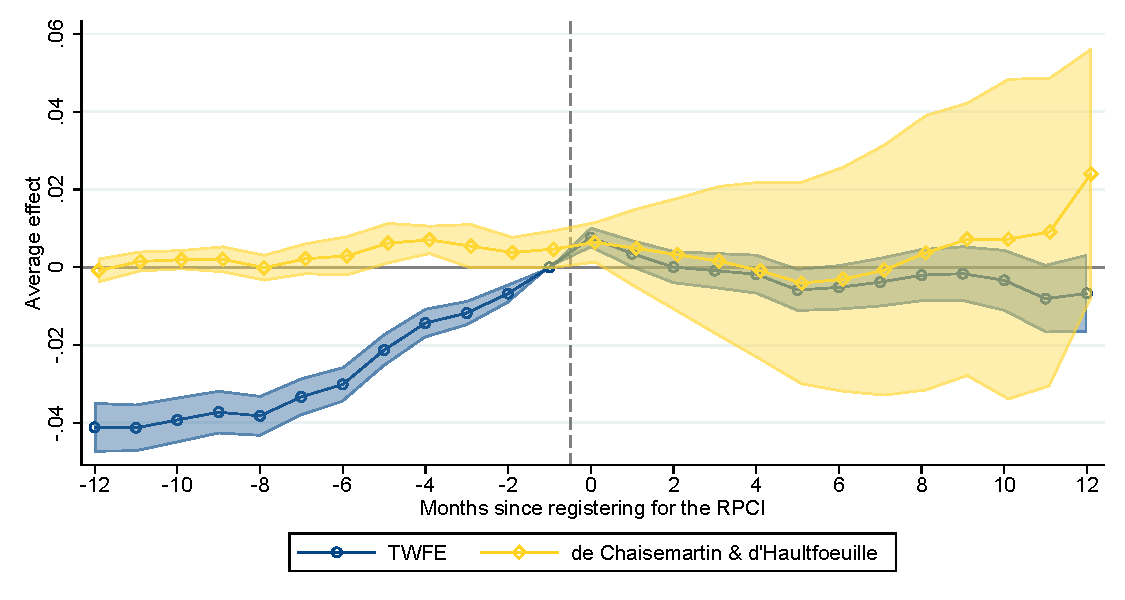
\includegraphics[width=\textwidth]{04_Figures/muestra_10porciento/event_study_alta_connected.pdf}
    \end{subfigure}
    \begin{subfigure}{0.49\textwidth}
    \caption{Effect on formal wage$^\dagger$}
    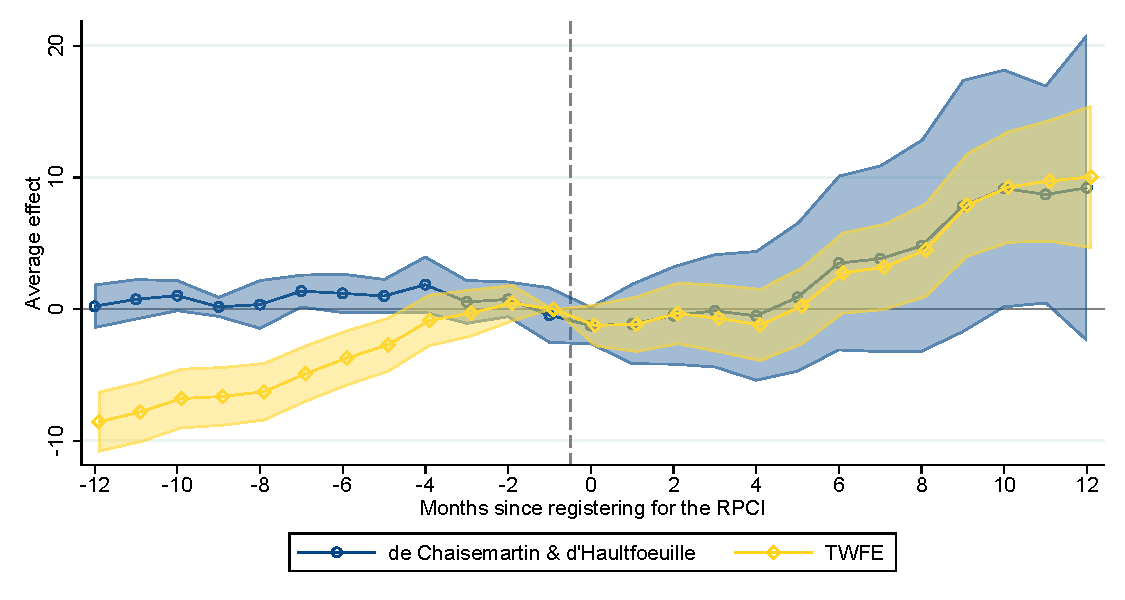
\includegraphics[width=\textwidth]{04_Figures/muestra_10porciento/event_study_sal_formal_connected.pdf}
    \end{subfigure}
    
    \begin{subfigure}{0.49\textwidth}
    \caption{Effect on wage}
    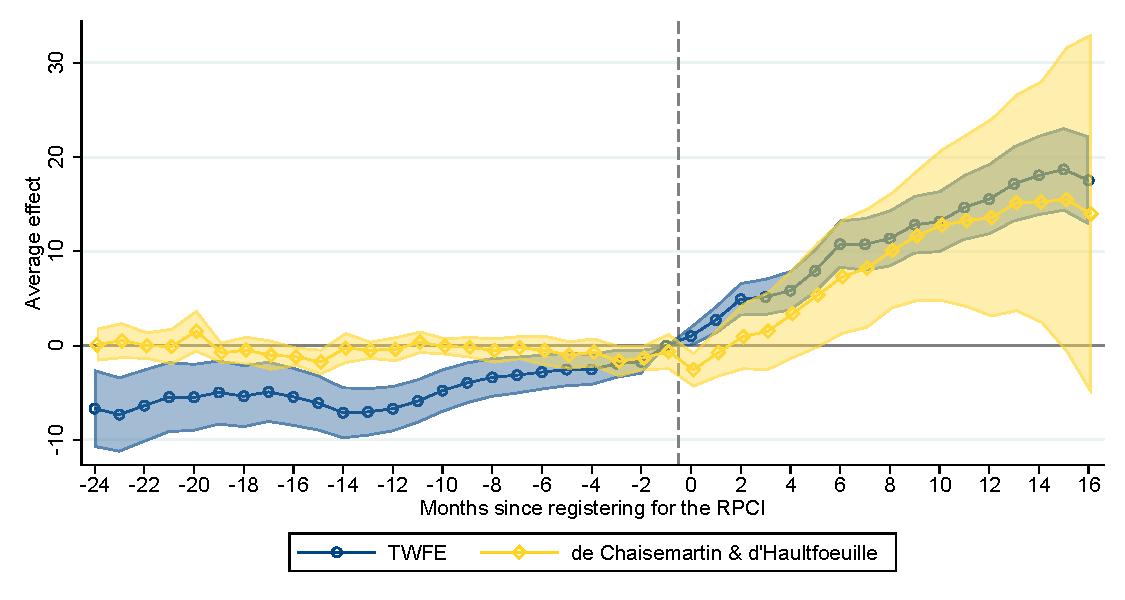
\includegraphics[width=\textwidth]{04_Figures/muestra_10porciento/event_study_sal_cierre_connected.pdf}
    \end{subfigure}
    \begin{subfigure}{0.49\textwidth}
    \caption{Effect on log wage}
    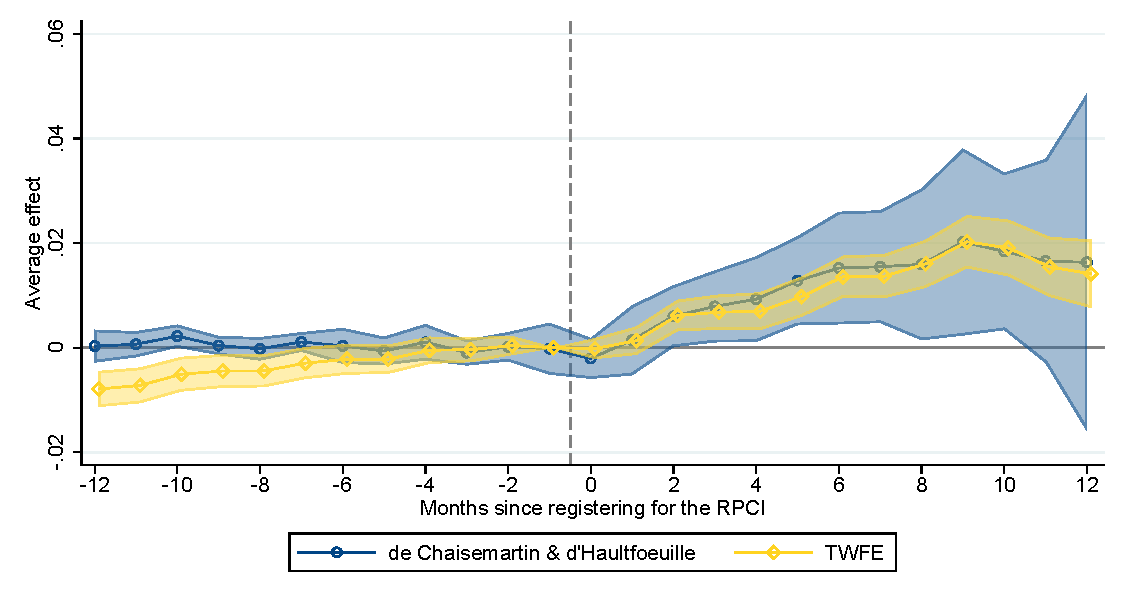
\includegraphics[width=\textwidth]{04_Figures/muestra_10porciento/event_study_log_sal_cierre_connected.pdf}
    \end{subfigure}
    
    %\textit{Do file: event_study_rpci.do}
\end{figure}

\scriptsize{
\noindent \textit{Notes}: This figure shows the event studies for the effect of registering to the RPCI on enrollment and the worker's wage. \textit{Sample:} Panel data for a random sample of the workers enrolled at the Mexican Institute of Social Security (IMSS) during 2020 and January 2021 (before the RPCI launch). \textit{Enrolled} is a dummy variable where 1 means worker $i$ was enrolled at IMSS during period $t$. $\dagger$ \textit{Formal Wage} and \textit{Wage} are the registered wage for worker $i$ during period $t$, the difference is \textit{Formal Wage} is 0 when the worker isn't enrolled, while \textit{Wage} is missing when the worker isn't enrolled. The lighter-shaded event studies present the estimators obtained from a TWFE specification. The darker-shaded event studies follow the estimators proposed by \cite{de2020two}, using the robust dynamic option to account for possible heterogeneous treatment effects across cohorts. Robust standard errors clustered by worker id. %This figure is referenced in \hyperref[subsec:workers]{Section} \ref{subsec:workers}.
} \\

\normalsize

\section{Heterogeneity by worker characteristics}

We also examine the heterogeneity of treatment effects based on worker and firm characteristics at baseline. Figure \ref{fig:heterogeneity_worker_rpci} displays the estimated coefficients obtained using the \cite{de2020two} specification, categorized by worker characteristics. The corresponding event studies for these estimates are presented in \ref{appendix_worker_char} \\

When considering gender, we observe a higher treatment effect on men's wages, while women experience a higher effect on log wages. This finding aligns with the fact that women generally earn lower wages than men. Despite the lower impact in monetary terms, the relative effect on women's wages could be proportionally higher due to their lower initial earnings. \\

Among young workers aged 25-35, a significant positive treatment effect is observed on formal wages, with significant effects on wages and log wages at a 10\% significance level. On the other hand, older workers nearing retirement age (65 years) exhibit interesting treatment effects: a negative impact on the probability of being enrolled, a negative effect on formal wages, and a positive effect on reported wages. These results suggest that older workers engage in crucial negotiations with their employers upon discovering their actual reported wage to IMSS, as their pension and retirement savings depend on this reported wage. \\

Additionally, we find a positive treatment effect for workers earning between 1 and 2 minimum wages, as well as those earning between 2 and 3 minimum wages. However, no significant effect is observed for workers with higher wages. This pattern is consistent with firms registering workers with the minimum possible wage or slightly above it. Notably, the highest effect on log wages is observed for workers earning between 1 and 2 minimum wages at baseline. Moreover, the event study examining the effect on wages for workers with baseline wages between 1 and 2 minimum wages reveals an approximate increase of $ \$30$ one year later. This increase accounts for nearly 18\% of the applicable minimum wage in 2022 ($\$172.87$), which is a substantial raise that is challenging to explain without potential underreporting by the employer. \\

\begin{figure}[H]
    \centering
    \caption{Heterogeneity by worker characteristics \label{fig:heterogeneity_worker_rpci}}
    
    \begin{subfigure}{\textwidth}
    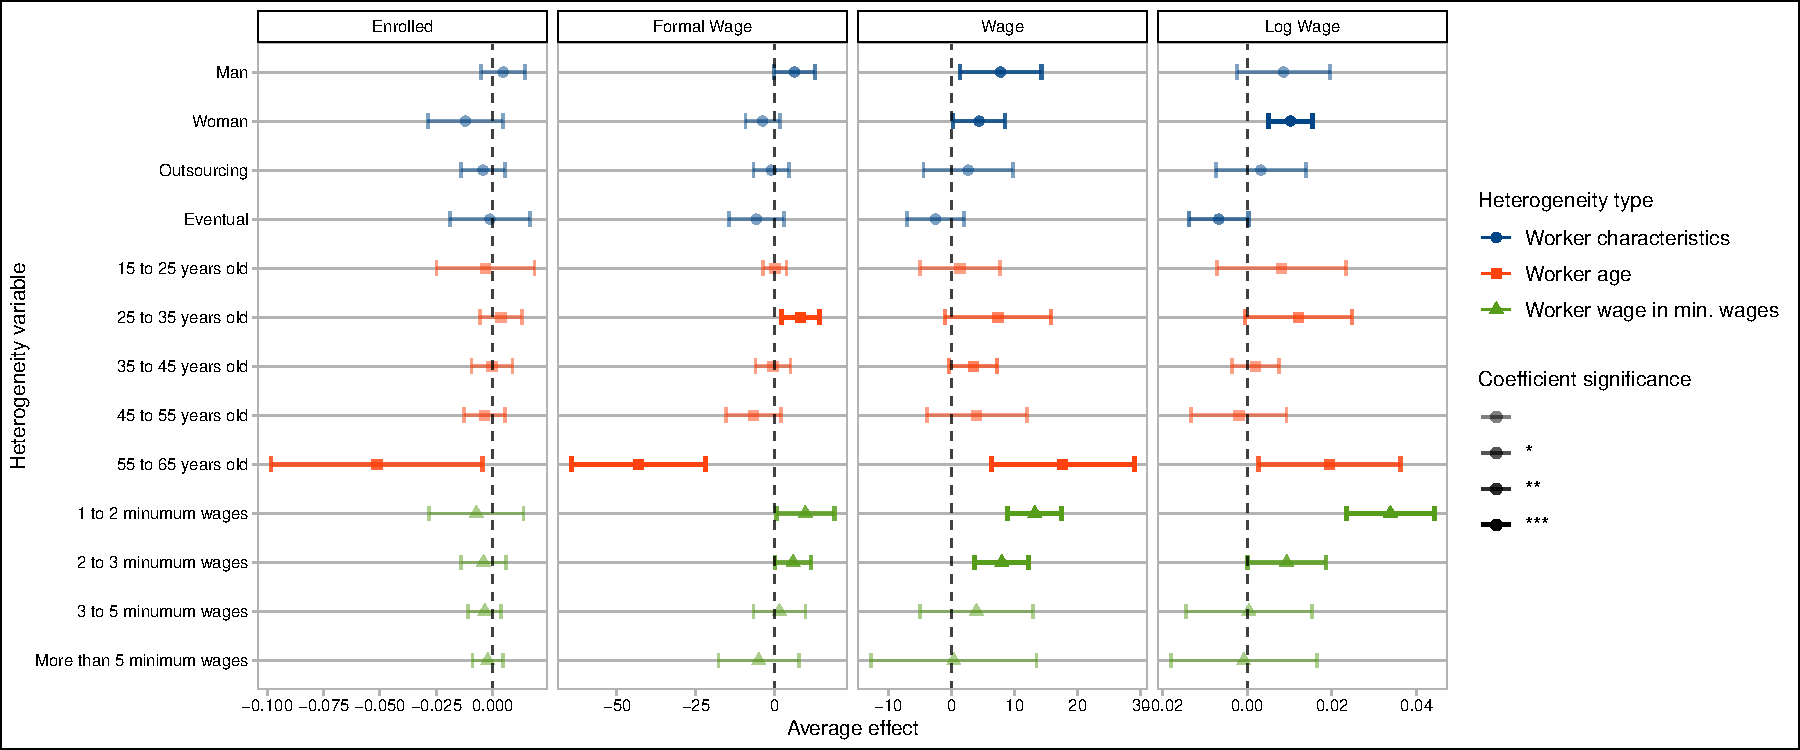
\includegraphics[width=\textwidth]{04_Figures/muestra_10porciento/dcdh_heterogeneity_worker_characteristics.pdf}
    \end{subfigure}
    
    %\textit{Do file: dcdh_heterogeneity_rpci.do}
\end{figure}

\scriptsize{
\noindent \textit{Notes}: This figure explores heterogeneity in the effect of registering to the RPCI on enrollment and the worker's wage by baseline worker's characteristics (characteristics during 2020, before the RPCI launch). \textit{Sample:} Panel data for a random sample of the workers enrolled at the Mexican Institute of Social Security (IMSS) during 2020 and January 2021 (before the RPCI launch). \textit{Enrolled} is a dummy variable where 1 means worker $i$ was enrolled at IMSS during period $t$. $\dagger$ \textit{Formal Wage} and \textit{Wage} are the registered wage for worker $i$ during period $t$, the difference is \textit{Formal Wage} is 0 when the worker isn't enrolled, while \textit{Wage} is missing when the worker isn't enrolled. The coefficient displayed is the average treatment effect estimated following \cite{de2020two}, using the robust dynamic option to account for possible heterogeneous treatment effects across cohorts. 95\% confidence intervals are shown. Robust standard errors clustered by worker id, with 250 bootstrap repetitions for the \cite{de2020two} estimator. *** $p<0.01$, ** $p<0.05$, * $p<0.1$. %This figure is referenced in %\hyperref[subsec:workers]{Section} \ref{subsec:workers}.
} \\

\normalsize

\section{Heterogeneity by firm characteristics}

Figure \ref{fig:heterogeneity_firm_rpci} displays the estimated coefficients by firm characteristics. The corresponding event studies for these estimates are provided in \ref{appendix_firm_char} \\

To examine the treatment effect based on job registers at IMSS, we distinguish between workers in the MX-USA border region and those away from the border. The border region is defined using INEGI's municipality identifiers, which align with the criteria used to establish differentiated minimum wages between the border and the rest of the country. We observe a positive treatment effect on wages for both groups, with a slightly higher point estimate along the border. However, the difference between the two estimates is not statistically significant. It is worth noting that the significance of both estimates may serve as a proxy for the significant impact on permanent jobs registered at IMSS since these are the jobs that have municipality identifiers. \\

Regarding regional analysis, we find a positive treatment effect on wages in the Central-West and North regions, with a stronger effect observed in the Central-West region. No effect for the South-East region. \\

Examining the treatment effect by firm industry, we observe positive effects on wages in the agriculture, construction, and services sectors, with the construction industry exhibiting the highest effect on log wages. \\

When considering firm size, we find a positive treatment effect on small firms (2-5 workers) and medium-sized firms (6-50 and 51-250 workers). This finding is consistent with previous research indicating a negative relationship between underreporting and firm size. \\

\begin{figure}[H]
    \centering
    \caption{Heterogeneity by firm characteristics \label{fig:heterogeneity_firm_rpci}}
    
    \begin{subfigure}{\textwidth}
    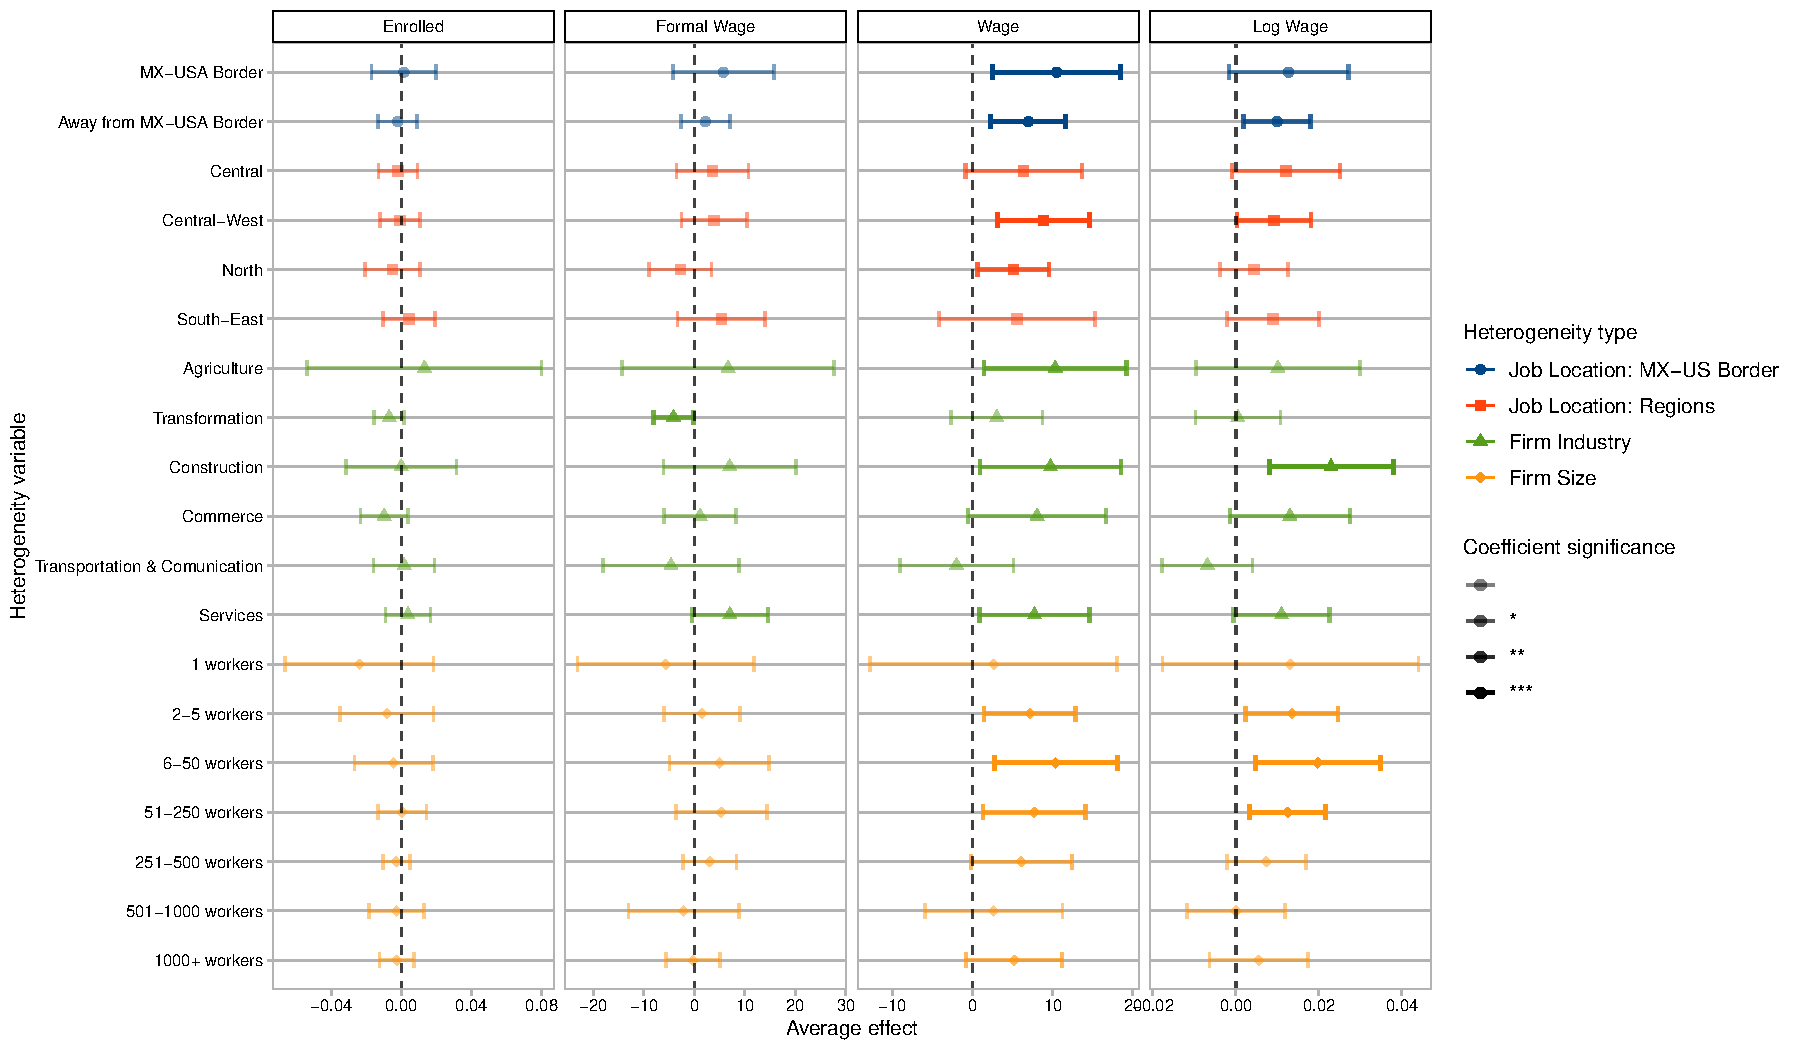
\includegraphics[width=\textwidth]{04_Figures/muestra_10porciento/dcdh_heterogeneity_firm_characteristics.pdf}
    \end{subfigure}
    
    %\textit{Do file: dcdh_heterogeneity_rpci.do}
\end{figure}

\scriptsize{
\noindent \textit{Notes}: This figure explores heterogeneity in the effect of registering to the RPCI on enrollment and the worker's wage by baseline firm's characteristics (characteristics during 2020, before the RPCI launch). \textit{Sample:} Panel data for a random sample of the workers enrolled at the Mexican Institute of Social Security (IMSS) during 2020 and January 2021 (before the RPCI launch). \textit{Enrolled} is a dummy variable where 1 means worker $i$ was enrolled at IMSS during period $t$. $\dagger$ \textit{Formal Wage} and \textit{Wage} are the registered wage for worker $i$ during period $t$, the difference is \textit{Formal Wage} is 0 when the worker isn't enrolled, while \textit{Wage} is missing when the worker isn't enrolled. The coefficient displayed is the average treatment effect estimated following \cite{de2020two}, using the robust dynamic option to account for possible heterogeneous treatment effects across cohorts. 95\% confidence intervals shown. Robust standard errors clustered by worker id, with 250 bootstrap repetitions for the \cite{de2020two} estimator. *** $p<0.01$, ** $p<0.05$, * $p<0.1$. %This figure is referenced in \hyperref[subsec:workers]{Section} \ref{subsec:workers}.
}

\normalsize

\section{Mechanisms}

We have established a positive causal effect of the RPCI on wages, but now we turn our attention to understanding how the RPCI impacts reported wages. Specifically, we aim to determine whether the increase in reported wages is occurring within a job or between jobs and whether collective bargaining between workers and employers drives the wage increments. It is important to note that the following analysis should not be interpreted as causal due to the presence of endogeneity. However, this section serves as a preliminary exploration of potential mechanisms and offers directions for future research. \\

To investigate whether the effect on wages occurs within a job or between jobs, we focused on two subsamples: workers who were consistently registered with the same employer throughout the sample period, and workers who were consistently enrolled at IMSS (regardless of the employer). By examining these subsamples, we aimed to identify any evidence of within-job wage increases or changes among workers who remained enrolled at IMSS. \\

Table \ref{twfe_wage_same_idrfc} presents the results of a simple TWFE regression for these subsamples. In both cases, we find a positive and significant coefficient on the RPCI variable. This suggests that the positive effect of the RPCI may partly stem from within-job wage increases. However, it is important to note that these results do not establish causality, and further analysis or data would be necessary to construct causal estimators specifically targeting within-job and between-job wage increments. \\

\begin{table}[H]
    \caption{RPCI effect on wage for workers with a unique employer and workers always employed}
    \label{twfe_wage_same_idrfc}
    \begin{center}
    \scriptsize{% Table generated by Excel2LaTeX from sheet 'twfe_wage_same'
\begin{tabular}{ccc}
\toprule
\toprule
      & Same Employer & Always Enrolled \\
      & (1)   & (2) \\
\cmidrule{2-3}      & \multicolumn{2}{c}{\textit{A) Wage}} \\
\midrule
RPCI  & 4.8*** & 7.1*** \\
      & (0.76) & (0.94) \\
Constant & 480.6*** & 539.4*** \\
      & (0.01) & (0.01) \\
Mean  & 480.6 & 539.5 \\
\cmidrule{2-3}      & \multicolumn{2}{c}{\textit{B) Log Wage}} \\
\midrule
RPCI  & 0.01*** & 0.02*** \\
      & (0.001) & (0.001) \\
Constant & 5.86*** & 5.98*** \\
      & (0.000) & (0.000) \\
Mean  & 5.86  & 5.98 \\
\midrule
Observations & 29,789,126 & 33,447,878 \\
Workers & 1,228,423 & 1,045,388 \\
Firms & 302,760 & 260,960 \\
\bottomrule
\bottomrule
\end{tabular}%
}
    %\textit{Do file: twfe_rpci.do}
    \end{center}
\end{table}

\scriptsize{
\noindent This table looks into the RPCI effect for workers with a single employer and workers always employed. Each column conditions a worker's job history throughout the sample. Column (1) conditions to workers with a single employer throughout the sample (these workers can be discharged and enrolled back as long as it's by the same employer). Column (2) conditions to workers always employed throughout the sample (these workers can change employers as long as they are always enrolled at IMSS). \textit{Sample:} Panel data for a random sample of the workers enrolled at the Mexican Institute of Social Security (IMSS) during 2020 and January 2021 (before the RPCI launch). Regressions use the TWFE specification $y_{it} = \gamma_{i} + \theta_{t}+ \beta RPCI_{it} +\epsilon_{it}$, where $\gamma_{i}$ are dummies for each worker id, $\theta_{t}$ are dummies for each monthly period, and $RPCI_{it}$ are dummies where 1 means that the worker registered for the RPCI during that month or previous month. Regressions include fixed effects on linear trends for age group, firm industry, state, and wage decile, by interacting dummies on worker's baseline characteristics with a set of dummies for each quarterly period. Robust standard errors clustered by worker id in parenthesis. *** $p<0.01$, ** $p<0.05$, * $p<0.1$.
} \\

\normalsize

Examining the potential spillover effects of the RPCI within a firm is indeed an interesting question. However, due to the potential correlation between the percentage of workers choosing to register for the RPCI within a firm and firm characteristics, traditional identification methods for estimating spillover effects may not provide accurate results. To address this issue, one possible solution is to implement a randomized control trial (RCT) design that explicitly randomizes the saturation of treatment. \\

In this RCT design, the saturation of treatment refers to the percentage of workers within a firm who register for the RPCI or are invited to register. By randomizing this saturation level, researchers can create a valid instrument to identify the spillover effects of the RPCI on outcomes. This approach allows for a more reliable estimation of the causal impact of the RPCI within a firm while mitigating potential biases that may arise from correlated firm characteristics. \\

The study conducted by \cite{vazquez2022identification} provides further insights and guidance on how to implement such an RCT design to accurately estimate spillover effects in the context of the RPCI. By adopting this methodology, researchers can generate more robust evidence regarding the spillover effects of the RPCI and contribute to our understanding of its broader impacts within firms. \\

To examine the correlation between the registration behavior within firms for the RPCI, you can conduct an analysis that investigates the relationship between your own registration for the RPCI in period $t+1$ and the registration behavior of others within your firm in period $t$. By including firm and period fixed effects, you can control for the intrinsic characteristics of the firm and period, isolating the correlation specific to the registration behavior.

In addition to analyzing whether someone within your firm registered for the RPCI in period $t$, you can extend the analysis by considering three other variables:

\begin{itemize}
    \item Percentage of workers in your firm who registered for the RPCI during period $t$ (excluding yourself): This variable captures the collective registration behavior within your firm, indicating the overall level of adoption of the RPCI.
    \item Presence of at least one worker already registered within your firm before period $t$: This variable examines whether the existence of prior registrations within your firm influences your decision to register for the RPCI.
    \item Percentage of workers in your firm who have already registered before period $t$ (excluding yourself): This variable reflects the historical registration pattern within your firm, indicating the extent of the previous adoption of the RPCI.
\end{itemize}

To analyze these relationships, you can run four separate specifications, incorporating the relevant variables and controlling for firm and period fixed effects. By doing so, you can assess the correlation between your own registration for the RPCI and the registration behavior within your firm, shedding light on potential social dynamics and peer effects influencing the decision to register for the program. \\

\begin{equation}
Register_{it+1} = \alpha + \lambda_j + \delta_t + \beta Register_{jt} + \epsilon_{it}
\end{equation}

\begin{equation}
Register_{it+1} = \alpha + \lambda_j + \delta_t + \beta Register_{jt} + \gamma Perc Register_{jt} + \epsilon_{it}
\end{equation}

\begin{equation}
Register_{it+1} = \alpha + \lambda_j + \delta_t + \beta RPCI_{jt} + \epsilon_{it}
\end{equation}

\begin{equation}
Register_{it+1} = \alpha + \lambda_j + \delta_t + \beta RPCI_{jt} + \gamma Perc RPCI_{jt} + \epsilon_{it}
\end{equation}

where:

\begin{itemize}
    \item $Register_{it+1}$ is a dummy where 1 means the worker $i$ registered for the RPCI during period $t+1$.
    \item $Register_{jt}$ is a dummy where 1 means that at least one worker other than worker $i$ that registered for the RPCI at firm $j$ (the firm worker $i$ is a registered employee) during period $t$.
    \item $PercRegister_{jt}$ is the percentage of workers other than worker $i$ that registered for the RPCI at firm $j$ (the firm worker $i$ is a registered employee) during period $t$.
    \item $RPCI_{jt}$ is a dummy where 1 means that at least one worker other than worker $i$ that registered for the RPCI at firm $j$ (the firm worker $i$ is a registered employee) during period $t$ or before.
    \item $PercRPCI_{jt}$ is the percentage of workers other than worker $i$ that registered for the RPCI at firm $j$ (the firm worker $i$ is a registered employee) during period $t$ or before.
    \item $\lambda_j$ are firm fixed effects.
    \item $\delta_t$ are period fixed effects.
\end{itemize}

Table \ref{tab:peer_rpci} presents the results from regressions examining the correlation between registering for the RPCI within my firm and my own likelihood of registering. The table shows a strong positive correlation for both the cumulative and instant registers at my firm during period $t$. Interestingly, this correlation is primarily driven by the percentage of coworkers who register for the RPCI at my firm, rather than simply the presence of at least one registration. These findings highlight the potential presence of spillover effects and the role of collective bargaining in an asymmetric information context. These are interesting results that could point to future research on the role of spillover effects or even collective bargaining in an asymmetric information context. \\

\begin{table}[H]
\footnotesize
\centering
\begin{threeparttable}
\centering
\caption{RPCI register spillover\label{tab:peer_rpci}}
%\textit{Do file: peer_rpci.do}

\begin{tabular}[t]{lcccc}
\toprule
\toprule
& \multicolumn{4}{c}{$Register_{it+1}$} \\
\midrule
\input 03_Tables/muestra_10porciento/peer_rpci

\bottomrule
\bottomrule

\end{tabular}

\begin{tablenotes}
\setlength\labelsep{0pt}
\scriptsize
\item \textit{Notes}: This table shows the correlation between registers for the RPCI within firms. \textit{Sample:} workers registered at a random sample of firms registered at the Mexican Institute of Social Security (IMSS) during January 2021, before the RPCI launch. \textit{Register$_{it}$} is a dummy variable which is 1 if the worker $i$ registered for the RPCI during period $t$. \textit{Register$_{jt}$} is a dummy which is 1 if at least one worker other than worker $i$ registered for the RPCI at firm $j$ (the firm worker $i$ is a registered employee) during period $t$. \textit{Register$_{jt}$ (\%)} is the percentage of workers other than worker $i$ that registered for the RPCI at firm $j$ (the firm worker $i$ is a registered employee) during period $t$. \textit{RPCI$_{jt}$} and \textit{RPCI$_{jt}$ (\%)} are the cumulative versions, meaning the register for the RPCI was during or before period $t$. Robust standard errors clustered by worker id in parenthesis. *** $p<0.01$, ** $p<0.05$, * $p<0.1$. %This table is referenced in \hyperref[subsec:peer]{Section} \ref{subsec:peer}.
\end{tablenotes}
\end{threeparttable}
\end{table}

\chapter{Conclusion} \label{conclusion}

In this study, we aimed to understand the effects of the RPCI (Reporte Personalizado de Cotizaciones en el IMSS) on wages and enrollment at IMSS. In this concluding chapter, we summarize our main findings, discuss their implications, and identify potential avenues for future research. \\

Our investigation consistently revealed a positive and significant treatment effect of the RPCI on wages. Both the simple two-way fixed effects (TWFE) specification and the \cite{de2020two} specification provided robust evidence of this impact. Moreover, our event studies demonstrated that the effect of the RPCI on wages increased over time, indicating dynamic effects that suggest potential long-term benefits for workers. These findings highlight the positive outcomes associated with formalization and compliance with labor regulations. \\

Furthermore, we explored the heterogeneity of treatment effects based on worker and firm characteristics. Our analysis showed variations in the impact of the RPCI across different groups. Gender was found to be a significant factor, with men and women experiencing different wage impacts. While the effect on pesos was lower for women, the relative impact was proportionally higher due to their lower initial wages. This emphasizes the importance of considering relative wage changes when evaluating policy interventions. \\

Age also played a role in the treatment effects of the RPCI. Younger workers (25-35 years) showed a significant positive treatment effect on formal wages, indicating potential benefits for individuals in the early stages of their careers. Interestingly, older workers nearing retirement age (65 years) displayed a negative treatment effect on the probability of being enrolled but a positive effect on reported wages. This suggests a unique break-or-make negotiation dynamic with employers as retirement savings depend on the reported wage. \\

Moreover, our analysis revealed that workers earning between 1 and 2 minimum wages at baseline experienced a considerable positive treatment effect. This suggests that firms tend to register workers with minimum possible wages or slightly above, and the highest impact on log wages was observed in this income bracket. Firm-level analyses also provided valuable insights, showing positive treatment effects in specific regions and industries. The MX-USA border region, the Central-West, and North regions exhibited significant treatment effects on wages. Among industries, positive effects were observed in agriculture, construction, and services, with the construction industry displaying the highest effect on log wages. Additionally, small and medium-sized firms (2-5 workers and 6-50, and 51-250 workers) demonstrated a positive treatment effect, aligning with prior research on the relationship between underreporting and firm size. \\

In our exploration of spillover effects within firms, we found a strong positive correlation between an individual's likelihood of registering for the RPCI and the registration behavior of their peers within the same firm. Specifically, the presence of more coworkers registering for the RPCI, rather than simply having at least one registration, influenced an individual's decision to enroll. This correlation suggests the existence of spillover effects and collective bargaining dynamics within firms, highlighting the role of information sharing and peer influence in the decision-making process. \\

While our study provides valuable insights, there are several avenues for future research to further enhance our understanding of the RPCI's effects on wages and firm behavior. First, causal estimators should be developed to investigate the mechanisms behind within and between job wage increments. Additionally, more rigorous identification strategies, such as randomized controlled trials, could be employed to accurately estimate spillover effects within firms. Further research is also needed to explore the underlying mechanisms driving the observed correlations, such as collective bargaining and asymmetric information dynamics. Longitudinal data and qualitative approaches could provide deeper insights into the long-term effects of the RPCI on workers, firms, and the overall labor market. Finally, comparative studies across different industries and countries would contribute to the generalizability of our findings. \\

In conclusion, our study sheds light on the effects of the RPCI on wages and firm behavior. The positive treatment effects underscore the potential benefits of formalization policies in improving working conditions and labor market outcomes. The heterogeneity of treatment effects based on worker and firm characteristics highlights the need for targeted interventions. Furthermore, the correlation within firms suggests the presence of spillover effects and collective bargaining dynamics, emphasizing the role of information sharing and peer influence in shaping individual decisions. Overall, our findings contribute to the ongoing dialogue surrounding labor market policies and call for further research in this important area of study. \\

%%%%%%%%%%%%%%%%%%%%%%%%%%%%%%%%%%%%%%%%%%%%%%%%%%%%%%%%%%%%%

\newpage

%%%%%%%%%%%%%%%%%%%%%%%%%%%%%%%%%%%%%%%%%%%%%%%%%%%%%%%%%%%%%
%BIBLIOGRAPHY

\clearpage
\bibliographystyle{ecta}
%\bibliographystyle{authordate1}
%\bibliographystyle{amsalpha}
%\bibliographystyle{AEA}

\bibliography{References}

%\FloatBarrier
%%%%%%%%%%%%%%%%%%%%%%%%%%%%%%%%%%%%%%%%

\clearpage
\singlespacing

\begin{comment}

\chapter{Tables}


\begin{table}[H]
\footnotesize
\centering
\begin{threeparttable}
\centering
\caption{Summary Statistics\label{tab:summary_stats_rpci}}
%\textit{Do file: summary_stats_rpci.do}

\begin{tabular}[t]{@{}l}
\toprule
\toprule
\begin{tabular}[t]{lccc}
\input 03_Tables/muestra_10porciento/summary_stats_rpci
\midrule
Workers & & & 1,412,210\\
Firms & & & 339,884\\
\end{tabular}

\tabularnewline 
\bottomrule
\bottomrule

\end{tabular}

\begin{tablenotes}
\setlength\labelsep{0pt}
\scriptsize
\item \textit{Notes}: This table shows summary statistics on selected variables for our final sample. \textit{Sample:} Panel data for a random sample of the workers enrolled at the Mexican Institute of Social Security (IMSS) during 2020 and January 2021 (before the RPCI launch). \textit{Registered for RPCI} is a dummy where 1 means worker $i$ registered for the RPCI at some point in our sample. \textit{Enrolled} is a dummy variable where 1 means worker $i$ was enrolled at IMSS during period $t$. \textit{Women}, \textit{Outsourcing} and \textit{Eventual} are dummies where 1 means worker $i$ is a woman, an outsourced worker or an eventual worker, respectively. \textit{Wage} is registered wage for worker $i$ during period $t$. \textit{N} is the number of non-missing observations for each variable. Wage and worker characteristics are only available if the worker was registered during period $t$. \textit{Workers} and \textit{Firms} are the number of unique workers and firms in our sample. This table is referenced in %\hyperref[subsec:workers]{Section} \ref{subsec:workers}.
\end{tablenotes}
\end{threeparttable}
\end{table}

\clearpage


\begin{table}[H]
\footnotesize
\centering
\begin{threeparttable}
\centering
\caption{RPCI effect on enrollment and wages\label{tab:dcdh_rpci}}
%\textit{Do file: event_study_rpci.do}

\begin{tabularx}{\textwidth}[t]{@{}l@{}l@{}l@{}l}
\toprule
\toprule
\multicolumn{4}{c}{\textit{Panel A:} TWFE} \\
\midrule
\begin{tabular}[t]{p{0.2\textwidth}P{0.15\textwidth}}
& Enrolled \\
\midrule
\input 03_Tables/muestra_10porciento/twfe_alta_wo_extended
\end{tabular}
&
\begin{tabular}[t]{HP{0.15\textwidth}}
& Formal Wage$^\dagger$ \\
\midrule
\input 03_Tables/muestra_10porciento/twfe_sal_formal_wo_extended
\end{tabular}
&
\begin{tabular}[t]{HP{0.15\textwidth}}
& Wage \\
\midrule
\input 03_Tables/muestra_10porciento/twfe_sal_cierre_wo_extended
\end{tabular}
&
\begin{tabular}[t]{HP{0.15\textwidth}}
& Log Wage \\
\midrule
\input 03_Tables/muestra_10porciento/twfe_log_sal_cierre_wo_extended
\end{tabular}
\end{tabularx}

\begin{tabularx}{\textwidth}[t]{@{}l@{}l@{}l@{}l}
\toprule
\toprule
\multicolumn{4}{c}{\textit{Panel B:} \cite{de2020two}} \\
\midrule
\begin{tabular}[t]{p{0.2\textwidth}P{0.15\textwidth}}
& Enrolled \\
\midrule
\input 03_Tables/muestra_10porciento/dcdh_alta
\end{tabular}
&
\begin{tabular}[t]{HP{0.15\textwidth}}
& Formal Wage$^\dagger$ \\
\midrule
\input 03_Tables/muestra_10porciento/dcdh_sal_formal
\end{tabular}
&
\begin{tabular}[t]{HP{0.15\textwidth}}
& Wage \\
\midrule
\input 03_Tables/muestra_10porciento/dcdh_sal_cierre
\end{tabular}
&
\begin{tabular}[t]{HP{0.15\textwidth}}
& Log Wage \\
\midrule
\input 03_Tables/muestra_10porciento/dcdh_log_sal_cierre
\end{tabular}

\tabularnewline 
\bottomrule
\bottomrule

\end{tabularx}

\begin{tablenotes}
\setlength\labelsep{0pt}
\scriptsize
\item \textit{Notes}: This table shows the effect of registering to the RPCI on enrollment and the worker's wage. \textit{Sample:} Panel data for a random sample of the workers enrolled at the Mexican Institute of Social Security (IMSS) during 2020 and January 2021 (before the RPCI launch). \textit{Enrolled} is a dummy variable where 1 means worker $i$ was enrolled at IMSS during period $t$. $\dagger$ \textit{Formal Wage} and \textit{Wage} are the registered wage for worker $i$ during period $t$, the difference is \textit{Formal Wage} is 0 when the worker isn't enrolled, while \textit{Wage} is missing when the worker isn't enrolled. \textit{Panel A} displays the coefficients obtained from simple TWFE specifications. \textit{Panel B} displays the average treatment effect estimated following \cite{de2020two}, using the robust dynamic option to account for possible heterogeneous treatment effects across cohorts. The number of observations in \textit{Panel B} is the number of differences between the outcome and the treatment used in the estimation. The effect is the average effect of the treatment across the switchers. Switchers are the number of switchers this effect applies to. Robust standard errors clustered by worker id in parenthesis. *** $p<0.01$, ** $p<0.05$, * $p<0.1$. This table is referenced in %\hyperref[subsec:workers]{Section} \ref{subsec:workers}.
\end{tablenotes}
\end{threeparttable}
\end{table}

\clearpage


\begin{comment}
\subsection{RPCI effect on wage changes}

\begin{table}[H]
\footnotesize
\centering
\begin{threeparttable}
\centering
\caption{RPCI effect on wage changes\label{tab:dcdh_wage_changes_rpci}}
%\textit{Do file: yearly_volatility_rpci.do}

\begin{tabularx}{0.75\textwidth}[t]{@{}l@{}l@{}l}
\toprule
\toprule
\begin{tabular}[t]{p{0.2\textwidth}P{0.15\textwidth}}
& Wage Changes \\
\midrule
\input 03_Tables/muestra_10porciento/dcdh_sal_diff_yr
\end{tabular}
&
\begin{tabular}[t]{HP{0.15\textwidth}}
& Wage Raises \\
\midrule
\input 03_Tables/muestra_10porciento/dcdh_sal_mayor_yr
\end{tabular}
&
\begin{tabular}[t]{HP{0.15\textwidth}}
& Wage Cuts \\
\midrule
\input 03_Tables/muestra_10porciento/dcdh_sal_menor_yr
\end{tabular}

\tabularnewline 
\bottomrule
\bottomrule

\end{tabularx}

\begin{tablenotes}
\setlength\labelsep{0pt}
\scriptsize
\item \textit{Notes}: This table shows the effect of registering to the RPCI on wage changes per year. \textit{Sample:} Panel data for a random sample of the workers enrolled at the Mexican Institute of Social Security (IMSS) during 2020 and January 2021 (before the RPCI launch). \textit{Wage Changes} counts the number of changes in the reported wage at IMSS of worker $i$ during year $t$. \textit{Wage Raises} counts the number of wage changes where the wage increased and \textit{Wage Cuts} counts the number of wage changes where the wage decreased. The coefficient displayed is the treatment effect on the year after being treated estimated following \cite{de2020two}. The number of observations are the number of differences of the outcome and of the treatment used in the estimation. The effect is the average effect of the treatment across the switchers. Switchers is the number of switchers this effect applies to. Robust standard errors clustered by worker id in parenthesis. *** $p<0.01$, ** $p<0.05$, * $p<0.1$. This table is referenced in %\hyperref[subsec:wage_changes]{Section} \ref{subsec:wage_changes}.
\end{tablenotes}
\end{threeparttable}
\end{table}
\clearpage


\singlespacing

\chapter{Figures}

%\subsection{Knowledge about IMSS}

\vspace{.7in}
\begin{figure}[H]
    \centering
    \caption{Knowledge about IMSS and worker's reported wages \label{fig:hist_knowledge_register_survey}}
    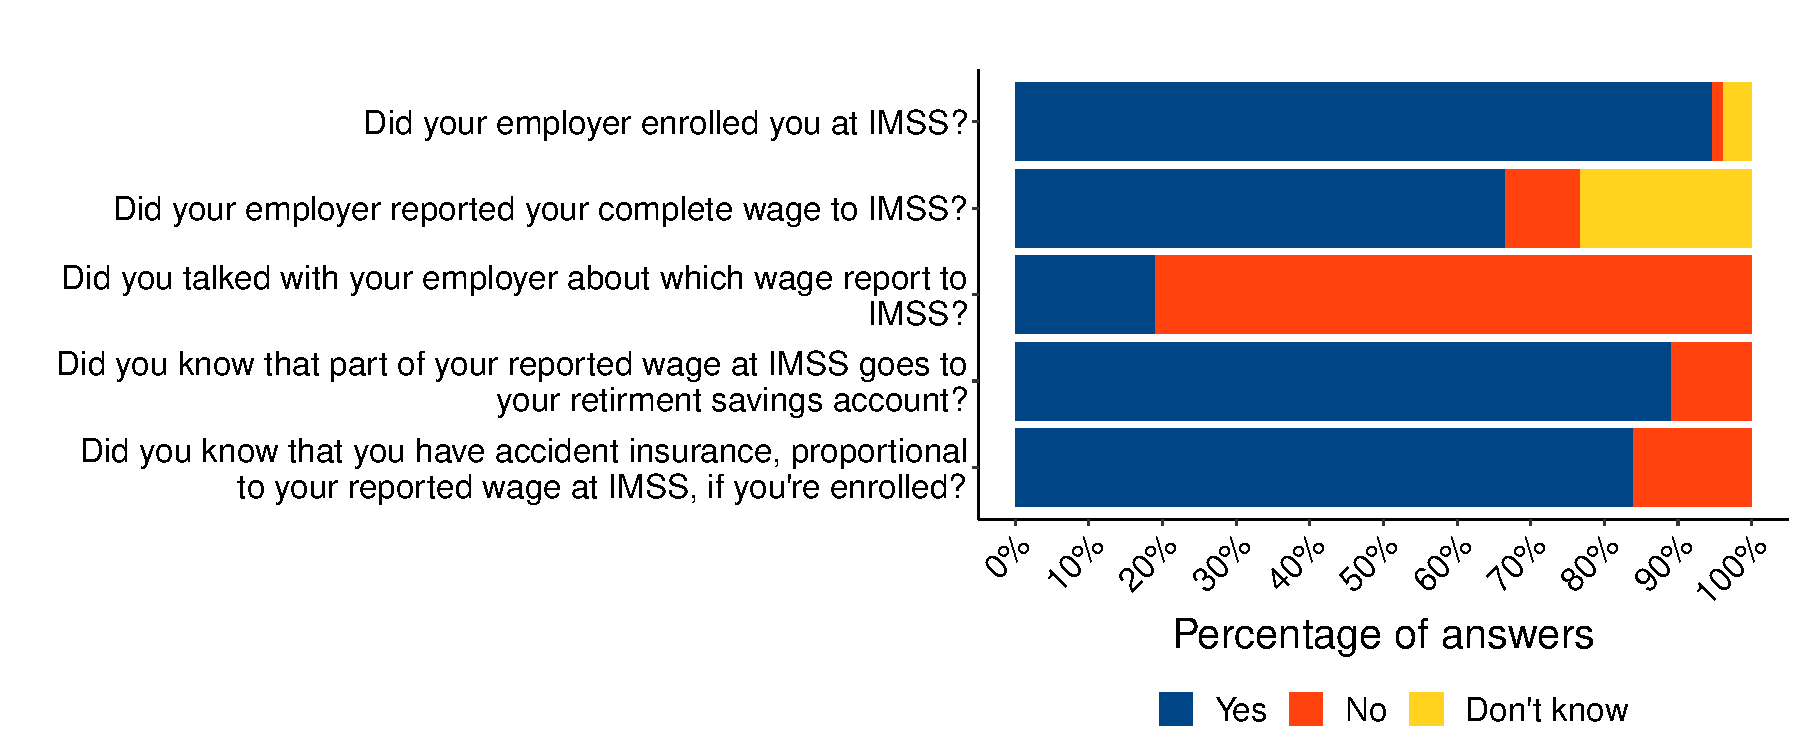
\includegraphics[width=\textwidth]{04_Figures/worker_survey/hist_knowledge_register_survey.pdf}
\end{figure}
\scriptsize{\textit{Notes}: This figure shows answers to questions about IMSS and wage reporting from the worker survey. \textit{Sample:} 233,709 answers from a survey conducted via email to workers enrolled at IMSS during August 2021. Questions 1-2, about the worker's employer, included the option "I don't know". Questions 3-5 ask about the worker's actions or knowledge didn't include the option "I don't know".}

\clearpage

%\subsection{RPCI}

\begin{figure}[H]
    \label{rpci_example}
    \caption{RPCI example}
    \begin{center}
    
    \begin{subfigure}{0.49\textwidth}
    \caption{RPCI within the IMSS Digital app}
    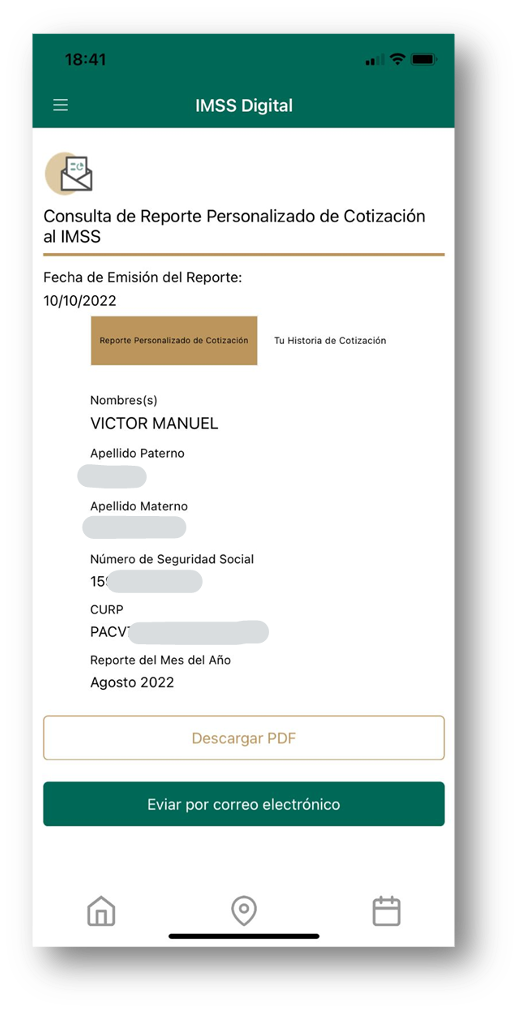
\includegraphics[width=\textwidth]{04_Figures/rpci_app/rpci_2.png}
    \end{subfigure}
    \begin{subfigure}{0.49\textwidth}
    \caption{RPCI PDF file}
    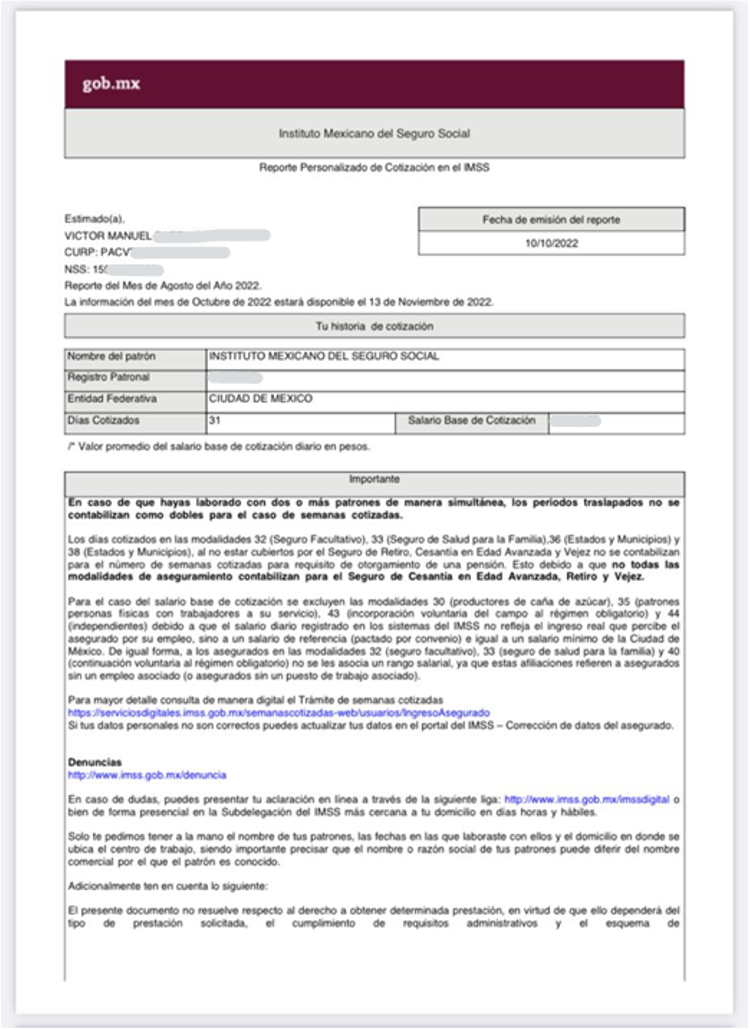
\includegraphics[width=\textwidth]{04_Figures/rpci_app/rpci_3.png}
    \end{subfigure}
    

    \end{center}
\end{figure}
\scriptsize{
\noindent Figure (a) shows the IMSS Digital app, where once the worker is registered for the RPCI, the worker can download their report in PDF or receive it via email. Figure (b) shows an example of the PDF for the RPCI. The report includes the worker job registered information, such as wage and the firm the worker is registered at.
}



%\subsection{RPCI registers by month}

\begin{figure}[H]
    \caption{RPCI registers by month}
    \label{hist_download}
    \begin{center}
    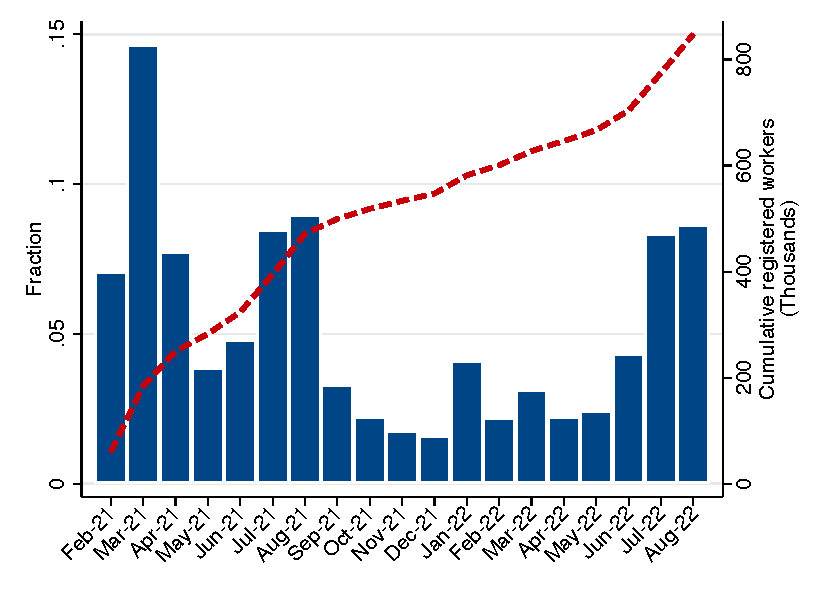
\includegraphics[width=0.65\textwidth]{04_Figures/muestra_1porciento/hist_download_month.pdf}
    \end{center}
\end{figure}
\scriptsize{
\noindent This figure shows the total number of workers registered for the RPCI. The right y-axis measures the fraction of workers who registered for the RPCI during each month from the total workers who registered for the RPCI. The left y-axis measures the cumulative number of workers who registered for the RPCI.
}

\clearpage

%\subsection{Event Studies: RPCI effect on enrollment and wages}

\begin{figure}[H]
    \centering
    \caption{Event studies - RPCI effect on enrollment and wages \label{fig:event_study_rpci}}
    
    \begin{subfigure}{0.49\textwidth}
    \caption{Effect on being enrolled}
    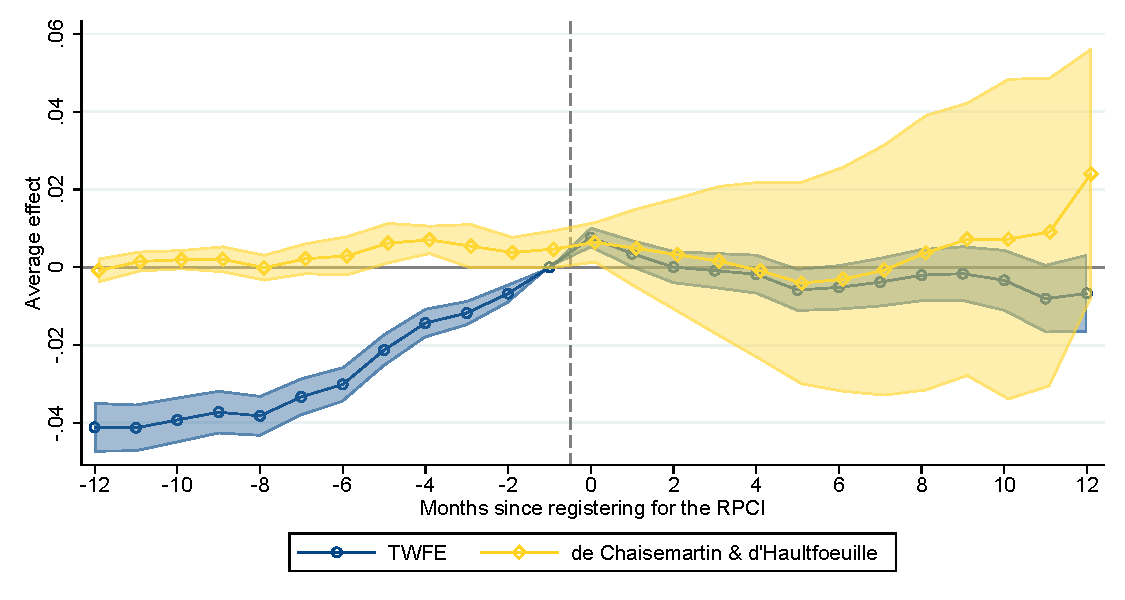
\includegraphics[width=\textwidth]{04_Figures/muestra_10porciento/event_study_alta_connected.pdf}
    \end{subfigure}
    \begin{subfigure}{0.49\textwidth}
    \caption{Effect on formal wage$^\dagger$}
    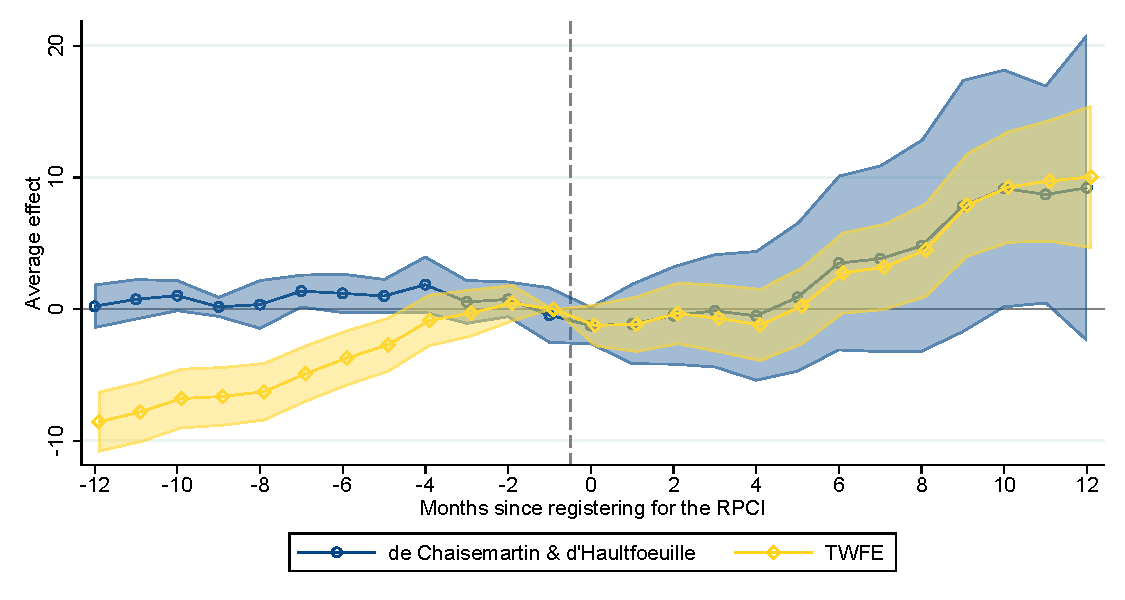
\includegraphics[width=\textwidth]{04_Figures/muestra_10porciento/event_study_sal_formal_connected.pdf}
    \end{subfigure}
    
    \begin{subfigure}{0.49\textwidth}
    \caption{Effect on wage}
    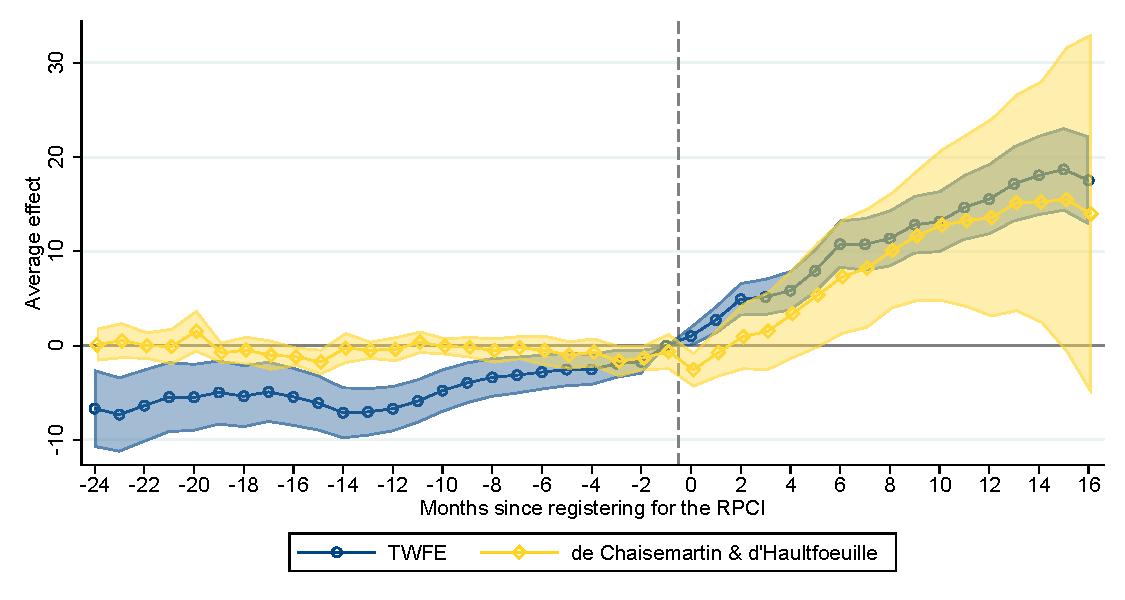
\includegraphics[width=\textwidth]{04_Figures/muestra_10porciento/event_study_sal_cierre_connected.pdf}
    \end{subfigure}
    \begin{subfigure}{0.49\textwidth}
    \caption{Effect on log wage}
    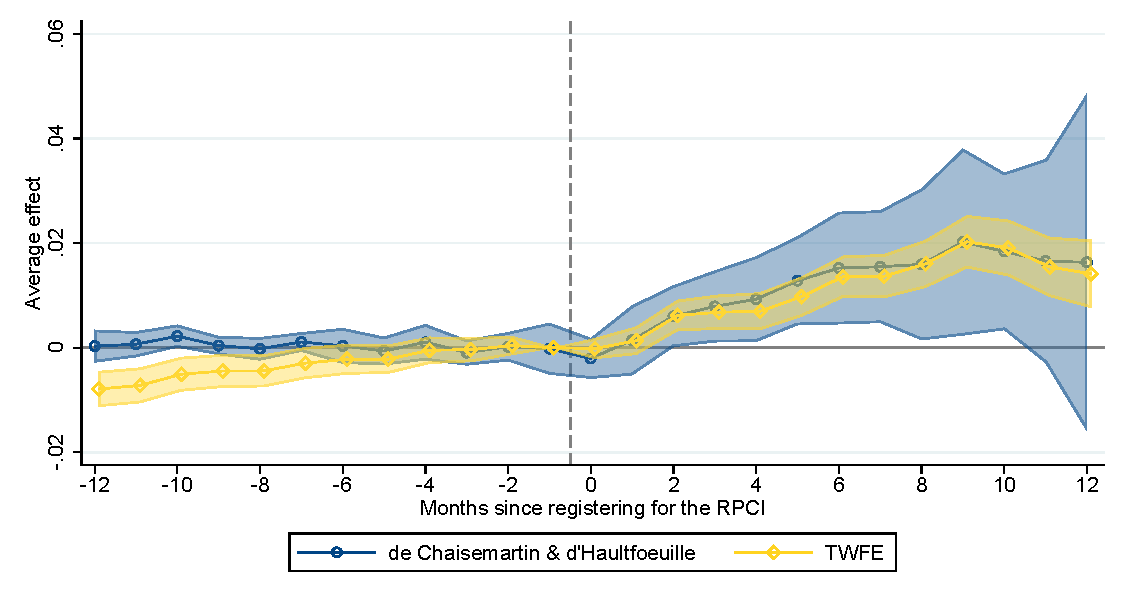
\includegraphics[width=\textwidth]{04_Figures/muestra_10porciento/event_study_log_sal_cierre_connected.pdf}
    \end{subfigure}
    
    %\textit{Do file: event_study_rpci.do}
\end{figure}

\scriptsize{
\noindent \textit{Notes}: This figure shows the event studies for the effect of registering to the RPCI on enrollment and the worker's wage. \textit{Sample:} Panel data for a random sample of the workers enrolled at the Mexican Institute of Social Security (IMSS) during 2020 and January 2021 (before the RPCI launch). \textit{Enrolled} is a dummy variable where 1 means worker $i$ was enrolled at IMSS during period $t$. $\dagger$ \textit{Formal Wage} and \textit{Wage} are the registered wage for worker $i$ during period $t$, the difference is \textit{Formal Wage} is 0 when the worker isn't enrolled, while \textit{Wage} is missing when the worker isn't enrolled. The lighter-shaded event studies present the estimators obtained from a TWFE specification. The darker-shaded event studies follow the estimators proposed by \cite{de2020two}, using the robust dynamic option to account for possible heterogeneous treatment effects across cohorts. Robust standard errors clustered by worker id. This figure is referenced in %\hyperref[subsec:workers]{Section} \ref{subsec:workers}.
}

\clearpage

\begin{comment}
    
%\subsection{Event Studies: RPCI effect on wage changes}

\begin{figure}[H]
    \centering
    \caption{Event studies - RPCI effect on wage changes \label{fig:event_study_wage_changes_rpci}}
    
    \begin{subfigure}{0.49\textwidth}
    \caption{Effect on wage changes}
    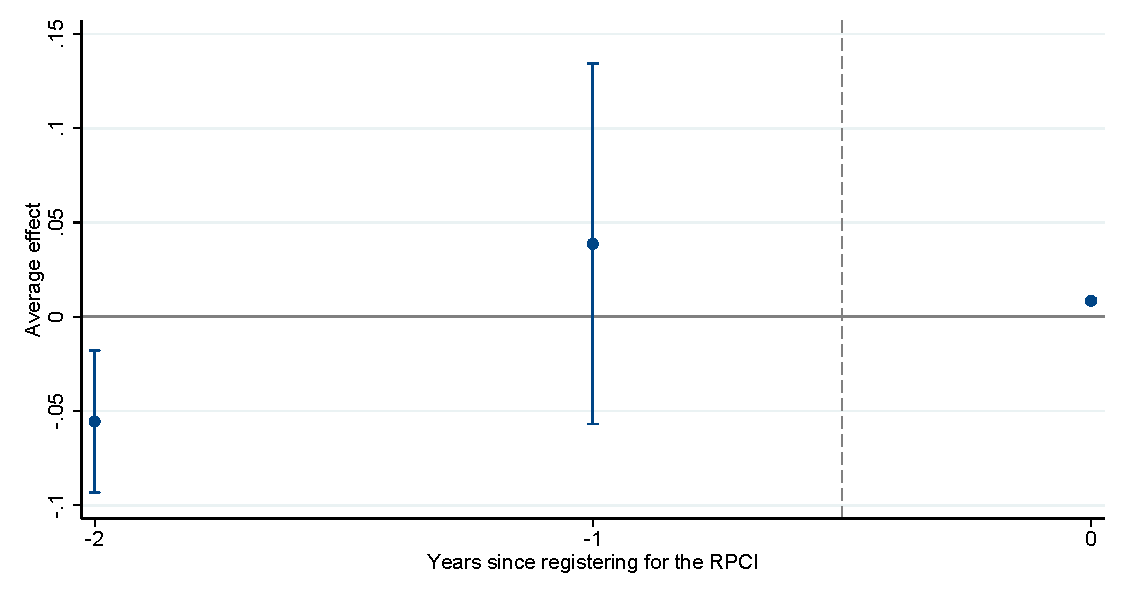
\includegraphics[width=\textwidth]{04_Figures/muestra_10porciento/event_study_sal_diff_yr_dcdh.pdf}
    \end{subfigure}
    
    \begin{subfigure}{0.49\textwidth}
    \caption{Effect on wage raises}
    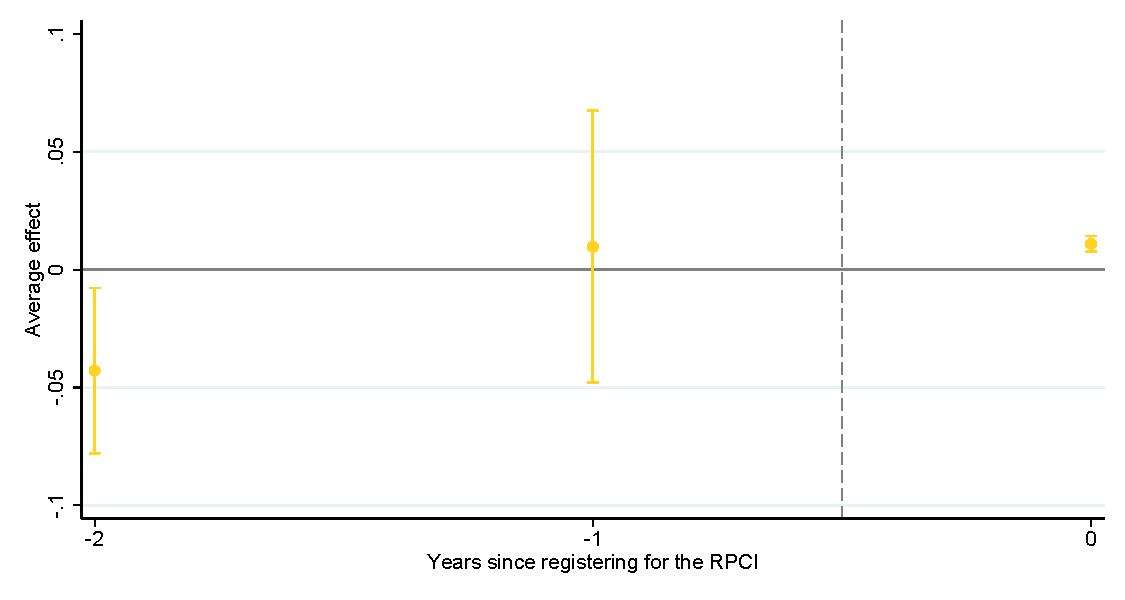
\includegraphics[width=\textwidth]{04_Figures/muestra_10porciento/event_study_sal_mayor_yr_dcdh.pdf}
    \end{subfigure}
    \begin{subfigure}{0.49\textwidth}
    \caption{Effect on wage cuts}
    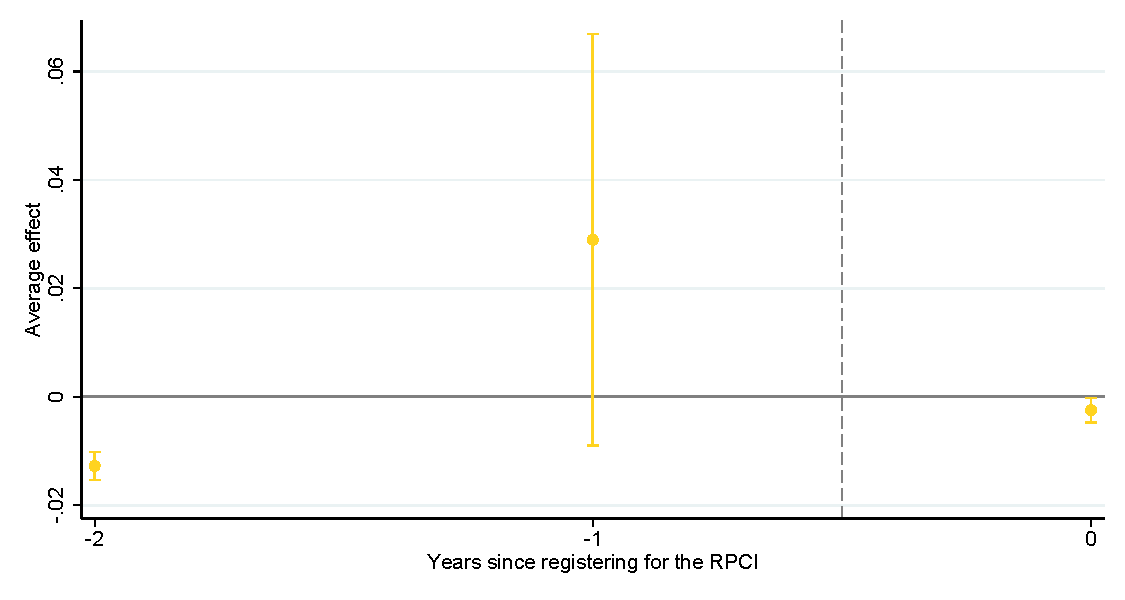
\includegraphics[width=\textwidth]{04_Figures/muestra_10porciento/event_study_sal_menor_yr_dcdh.pdf}
    \end{subfigure}
    
    %\textit{Do file: event_study_rpci.do}
\end{figure}

\scriptsize{
\noindent \textit{Notes}: This figures shows the event studies for the effect of registering to the RPCI on enrollment and the worker's wage. \textit{Sample:} Panel data for a random sample of the workers enrolled at the Mexican Institute of Social Security (IMSS) during during 2020 and January 2021 (before the RPCI launch). \textit{Wage Changes} counts the number of changes in the reported wage at IMSS of worker $i$ during year $t$. \textit{Wage Raises} counts the number of wage changes where the wage increased and \textit{Wage Cuts} counts the number of wage changes where the wage decreased. The event studies follow the estimators proposed by \cite{de2020two}, using the robust dynamic option to account for possible heterogeneous treatment effects across cohorts. Robust standard errors clustered by worker id. This figure is referenced in %\hyperref[subsec:workers]{Section} \ref{subsec:workers}.
}

%\subsection{Heterogeneity by worker characteristics}

\begin{figure}[H]
    \centering
    \caption{Heterogeneity by worker characteristics \label{fig:heterogeneity_worker_rpci}}
    
    \begin{subfigure}{\textwidth}
    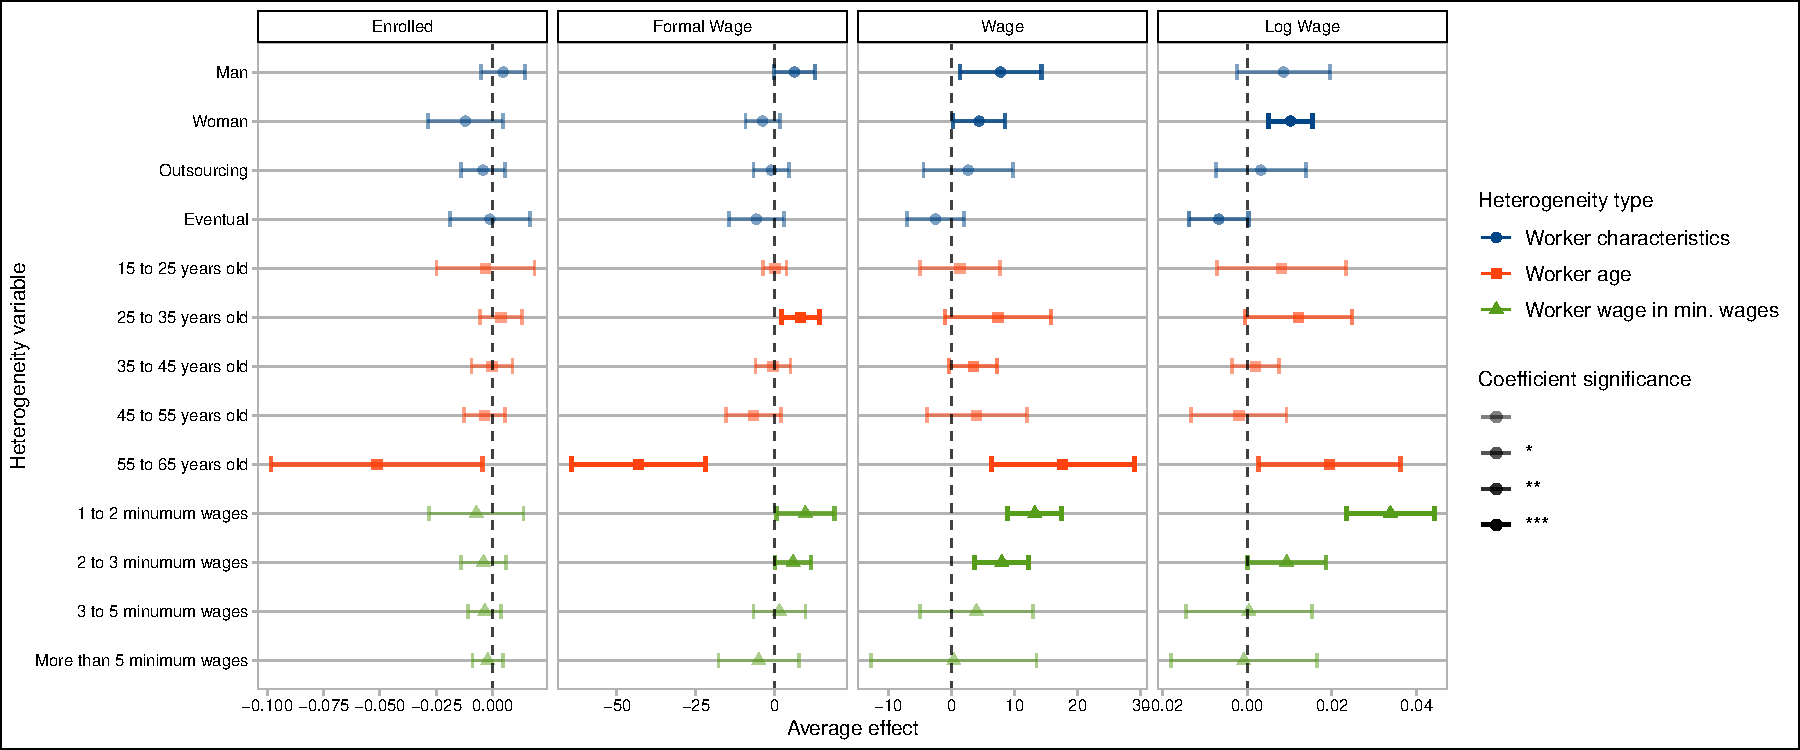
\includegraphics[width=\textwidth]{04_Figures/muestra_10porciento/dcdh_heterogeneity_worker_characteristics.pdf}
    \end{subfigure}
    
    %\textit{Do file: dcdh_heterogeneity_rpci.do}
\end{figure}

\scriptsize{
\noindent \textit{Notes}: This figure explores heterogeneity in the effect of registering to the RPCI on enrollment and the worker's wage by baseline worker's characteristics (characteristics during 2020, before the RPCI launch). \textit{Sample:} Panel data for a random sample of the workers enrolled at the Mexican Institute of Social Security (IMSS) during 2020 and January 2021 (before the RPCI launch). \textit{Enrolled} is a dummy variable where 1 means worker $i$ was enrolled at IMSS during period $t$. $\dagger$ \textit{Formal Wage} and \textit{Wage} are the registered wage for worker $i$ during period $t$, the difference is \textit{Formal Wage} is 0 when the worker isn't enrolled, while \textit{Wage} is missing when the worker isn't enrolled. The coefficient displayed is the average treatment effect estimated following \cite{de2020two}, using the robust dynamic option to account for possible heterogeneous treatment effects across cohorts. 95\% confidence intervals are shown. Robust standard errors clustered by worker id. *** $p<0.01$, ** $p<0.05$, * $p<0.1$. %This figure is referenced in %\hyperref[subsec:workers]{Section} \ref{subsec:workers}.
}

\clearpage

%\subsection{Heterogeneity by firm characteristics}

\begin{figure}[H]
    \centering
    \caption{Heterogeneity by firm characteristics \label{fig:heterogeneity_firm_rpci}}
    
    \begin{subfigure}{\textwidth}
    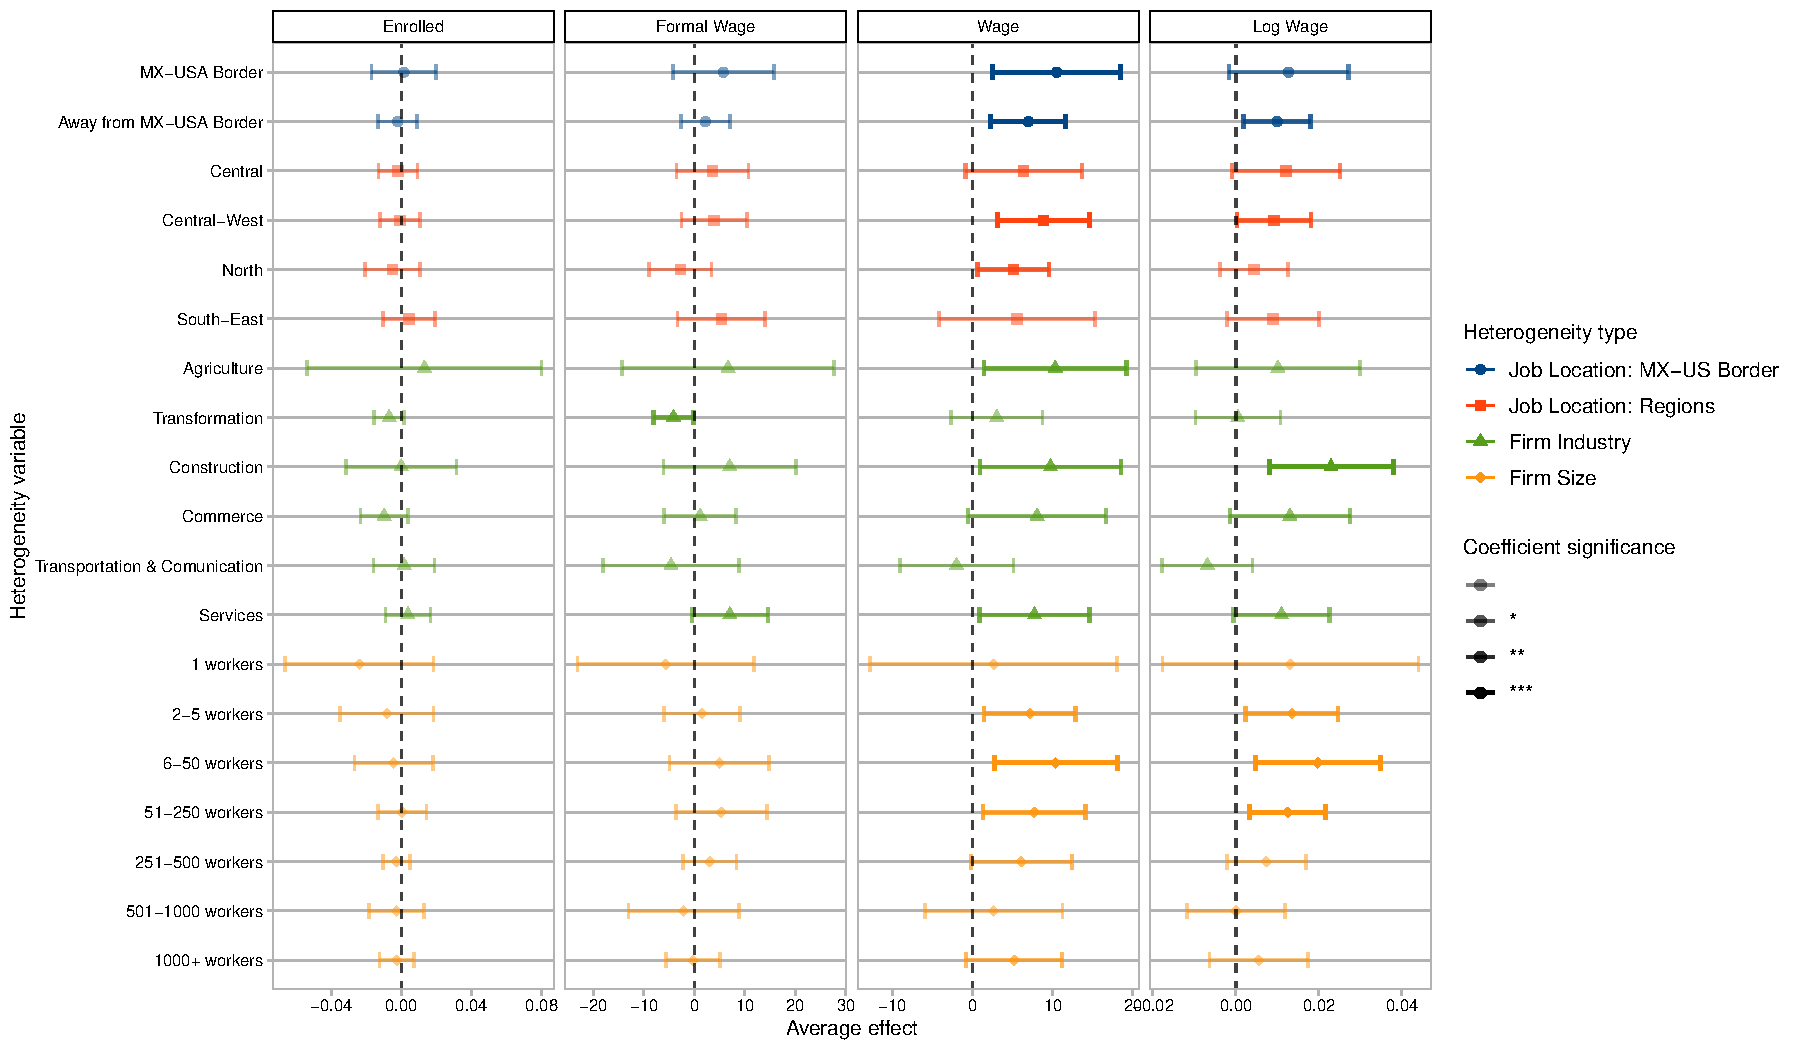
\includegraphics[width=\textwidth]{04_Figures/muestra_10porciento/dcdh_heterogeneity_firm_characteristics.pdf}
    \end{subfigure}
    
    %\textit{Do file: dcdh_heterogeneity_rpci.do}
\end{figure}

\scriptsize{
\noindent \textit{Notes}: This figure explores heterogeneity in the effect of registering to the RPCI on enrollment and the worker's wage by baseline firm's characteristics (characteristics during 2020, before the RPCI launch). \textit{Sample:} Panel data for a random sample of the workers enrolled at the Mexican Institute of Social Security (IMSS) during 2020 and January 2021 (before the RPCI launch). \textit{Enrolled} is a dummy variable where 1 means worker $i$ was enrolled at IMSS during period $t$. $\dagger$ \textit{Formal Wage} and \textit{Wage} are the registered wage for worker $i$ during period $t$, the difference is \textit{Formal Wage} is 0 when the worker isn't enrolled, while \textit{Wage} is missing when the worker isn't enrolled. The coefficient displayed is the average treatment effect estimated following \cite{de2020two}, using the robust dynamic option to account for possible heterogeneous treatment effects across cohorts. 95\% confidence intervals shown. Robust standard errors clustered by worker id. *** $p<0.01$, ** $p<0.05$, * $p<0.1$. This figure is referenced in %\hyperref[subsec:workers]{Section} \ref{subsec:workers}.
}

\clearpage

\end{comment}

%%%%%%%%%%%%%%%%%%%%%%%%%%%%%%%%%%%%%%%%%%%%%%%%%%%%%%

\newpage
%  \documentclass[oneside,11pt]{article}

% 
\usepackage{soul}
\usepackage{natbib}
\usepackage{hyperref}
\usepackage{bookmark}
\usepackage{graphicx}             
\graphicspath{{./Figuras/}}
\usepackage[dvipsnames]{xcolor}
\usepackage{todonotes}
\usepackage{makecell}
\usepackage[margin=1in]{geometry}
\usepackage{float}                
\usepackage{amsmath}
\usepackage{amscd}
\usepackage{amsfonts}
\usepackage{amssymb}
\usepackage{bbm}
\usepackage{booktabs}
\usepackage{nameref}
\usepackage{multirow}
\usepackage[nokeyprefix]{refstyle}
\usepackage{rotating}
\usepackage{threeparttable}
\usepackage{afterpage}
\usepackage{lscape}
\usepackage{enumerate}
\usepackage{caption}
\usepackage{subcaption}
\usepackage{epstopdf}
\usepackage{setspace}
\usepackage{svg}
\usepackage{dsfont}
\usepackage{amsthm}
\usepackage{tocloft}
\usepackage{etoc}
\usepackage{lmodern}
\usepackage{bm}
\usepackage[T1]{fontenc}
\usepackage{tgpagella}

\epstopdfDeclareGraphicsRule{.tiff}{png}{.png}{convert #1 \OutputFile}
\AppendGraphicsExtensions{.tiff}

\epstopdfDeclareGraphicsRule{.tif}{png}{.png}{convert #1 \OutputFile}
\AppendGraphicsExtensions{.tif}

\def\sym#1{\ifmmode^{#1}\else\(^{#1}\)\fi}

\usepackage{tikz}
\usetikzlibrary{shapes.geometric, arrows}
\usetikzlibrary{calc}
\usetikzlibrary{matrix}

\tikzset{ 
    table/.style={
        matrix of nodes,
        row sep=-\pgflinewidth,
        column sep=-\pgflinewidth,
        nodes={
            rectangle,
            draw=black,
            align=center
        },
        minimum height=1.5em,
        text depth=0.5ex,
        text height=2ex,
        nodes in empty cells,
%%
        every even row/.style={
            nodes={fill=gray!20}
        },
        column 1/.style={
            nodes={text width=2em,font=\bfseries}
        },
        row 1/.style={
            nodes={
                fill=black,
                text=white,
                font=\bfseries
            }
        }
    }
}


\usepackage{colortbl}
\usepackage{url}
\urlstyle{rm}
\definecolor{darkblue}{rgb}{0,0,.4}
\hypersetup{colorlinks=true, breaklinks=true, citecolor=Maroon, linkcolor=darkblue, menucolor=darkblue, urlcolor=darkblue}

\newtheorem{theorem}{Theorem}
\newtheorem{claim}[theorem]{Claim}
\newtheorem{prop}[theorem]{Proposition} 
\newtheorem{cor}[theorem]{Corollary} 
\newtheorem{assumption}{Assumption} 
\newtheorem{lem}{Lemma} 

\DeclareRobustCommand{\hlgr}[1]{{\sethlcolor{green}\hl{#1}}}


\usepackage{comment}
%para esconder columnas en tablas (enrique)
\usepackage{array}
\newcolumntype{H}{>{\setbox0=\hbox\bgroup}c<{\egroup}@{}}
\linespread{1.25}

\newcommand{\wh}{\widehat}
\usepackage{anyfontsize}

\usepackage[linesnumbered,vlined,ruled,commentsnumbered]{algorithm2e}

\DontPrintSemicolon
\newcommand{\To}{\mbox{\upshape\bfseries to}}
\newcommand{\E}{\mathbb{E}}

\DeclareCaptionFormat{cont}{#1 (cont.)#2#3\par}
% %%% HELPER CODE FOR DEALING WITH EXTERNAL REFERENCES
% \usepackage{xr}
% \makeatletter
% \newcommand*{\addFileDependency}[1]{
%   \typeout{(#1)}
%   \@addtofilelist{#1}
%   \IfFileExists{#1}{}{\typeout{No file #1.}}
% }
% \makeatother


% \newcommand*{\myexternaldocument}[1]{
%     \externaldocument{#1}
%     \addFileDependency{#1.tex}
%     \addFileDependency{#1.aux}
% }

% %\myexternaldocument{OA}

% %%%%%%%%%%%%%%%%%%%%%%%%%%%%%%%% DOCUMENT
% \begin{document}

%%%%%%%%%%%%%%%%%%%%%%%%%%%%%%%%%%%%%%%%%%%%%%%

% APPENDIX 
\setcounter{table}{0}
\setcounter{figure}{0}
\setcounter{section}{0}
\pagenumbering{gobble}


\begin{center}
	\LARGE IMSS RPCI \\[0.5em]
	\Large{Appendix $-$ For Online Publication} \\[1em]
	\large \author{Eduardo Alcaraz \and Gabriela López \and Luis Martínez \and Marco Medina \and Enrique Seira}
\end{center}

\appendix
\pagenumbering{arabic}
\renewcommand\thefigure{OA-\arabic{figure}}
\renewcommand\thetable{OA-\arabic{table}}
\renewcommand*{\thepage}{OA - \arabic{page}}
\renewcommand\thesection{Appendix \Alph{section}.}
\renewcommand\thesubsection{\Alph{section}.\arabic{subsection}}

%\renewcommand{\cftparskip}{0em} % NOT NEEDED
\renewcommand\cftsecdotsep{\cftdotsep}
\renewcommand\cftsubsecdotsep{\cftnodots}
\renewcommand{\cftsecnumwidth}{6em}
 \renewcommand{\cftpnumalign}{r}
%\renewcommand{\cftsecleader}{\normalfont\cftdotfill{\cftsecdotsep}}


\renewcommand{\cftsecleader}{\cftdotfill{\cftsecdotsep}\hspace{1.8em}}
%\renewcommand{\cftsecpagefont}{20em}
%\renewcommand{\cftfignumwidth}{6em}
%\renewcommand{\cfttabnumwidth}{3.3em}

%\tableofcontents
\etocdepthtag.toc{mtappendix}
\etocsettagdepth{mtchapter}{none}
\etocsettagdepth{mtappendix}{subsection}

\setstretch{0.9}
%\renewcommand\contentsname{} % the empty name

\begingroup
\let\clearpage\relax
%\vspace{-1.5em} % the removed space. Set as appropriate
\tableofcontents
\endgroup

\clearpage

\section{ RPCI}
\vspace{.2in}

\begin{figure}[H]
    \caption{RPCI flyers}
    \label{rpci_flyers}
    \begin{center}
    
    \begin{subfigure}{0.49\textwidth}
    \caption{RPCI flyer titled "Does my employer has me registered at IMSS?"}
    
\includegraphics[width=\textwidth]{04_Figures/rpci_app/rpci_flyer_3.jpeg}
    \end{subfigure}
    \begin{subfigure}{0.49\textwidth}
    \caption{RPCI flyer titled "Digital services for a healthy environment"}
    
\includegraphics[width=\textwidth]{04_Figures/rpci_app/rpci_flyer_2.jpeg}
    \end{subfigure}

    \end{center}
\end{figure}
\scriptsize{
\noindent Flyers circulated by the Mexican Institute of Social Security (IMSS) for the RPCI. Both flyers explain how you can track and access your job register information, such as wage and firm you are registered at, if you register for the RPCI.
}

\clearpage

\begin{figure}[H]
    \caption{Registering for the RPCI}
    \label{rpci_register}
    \begin{center}
    
    \begin{subfigure}{0.9\textwidth}
    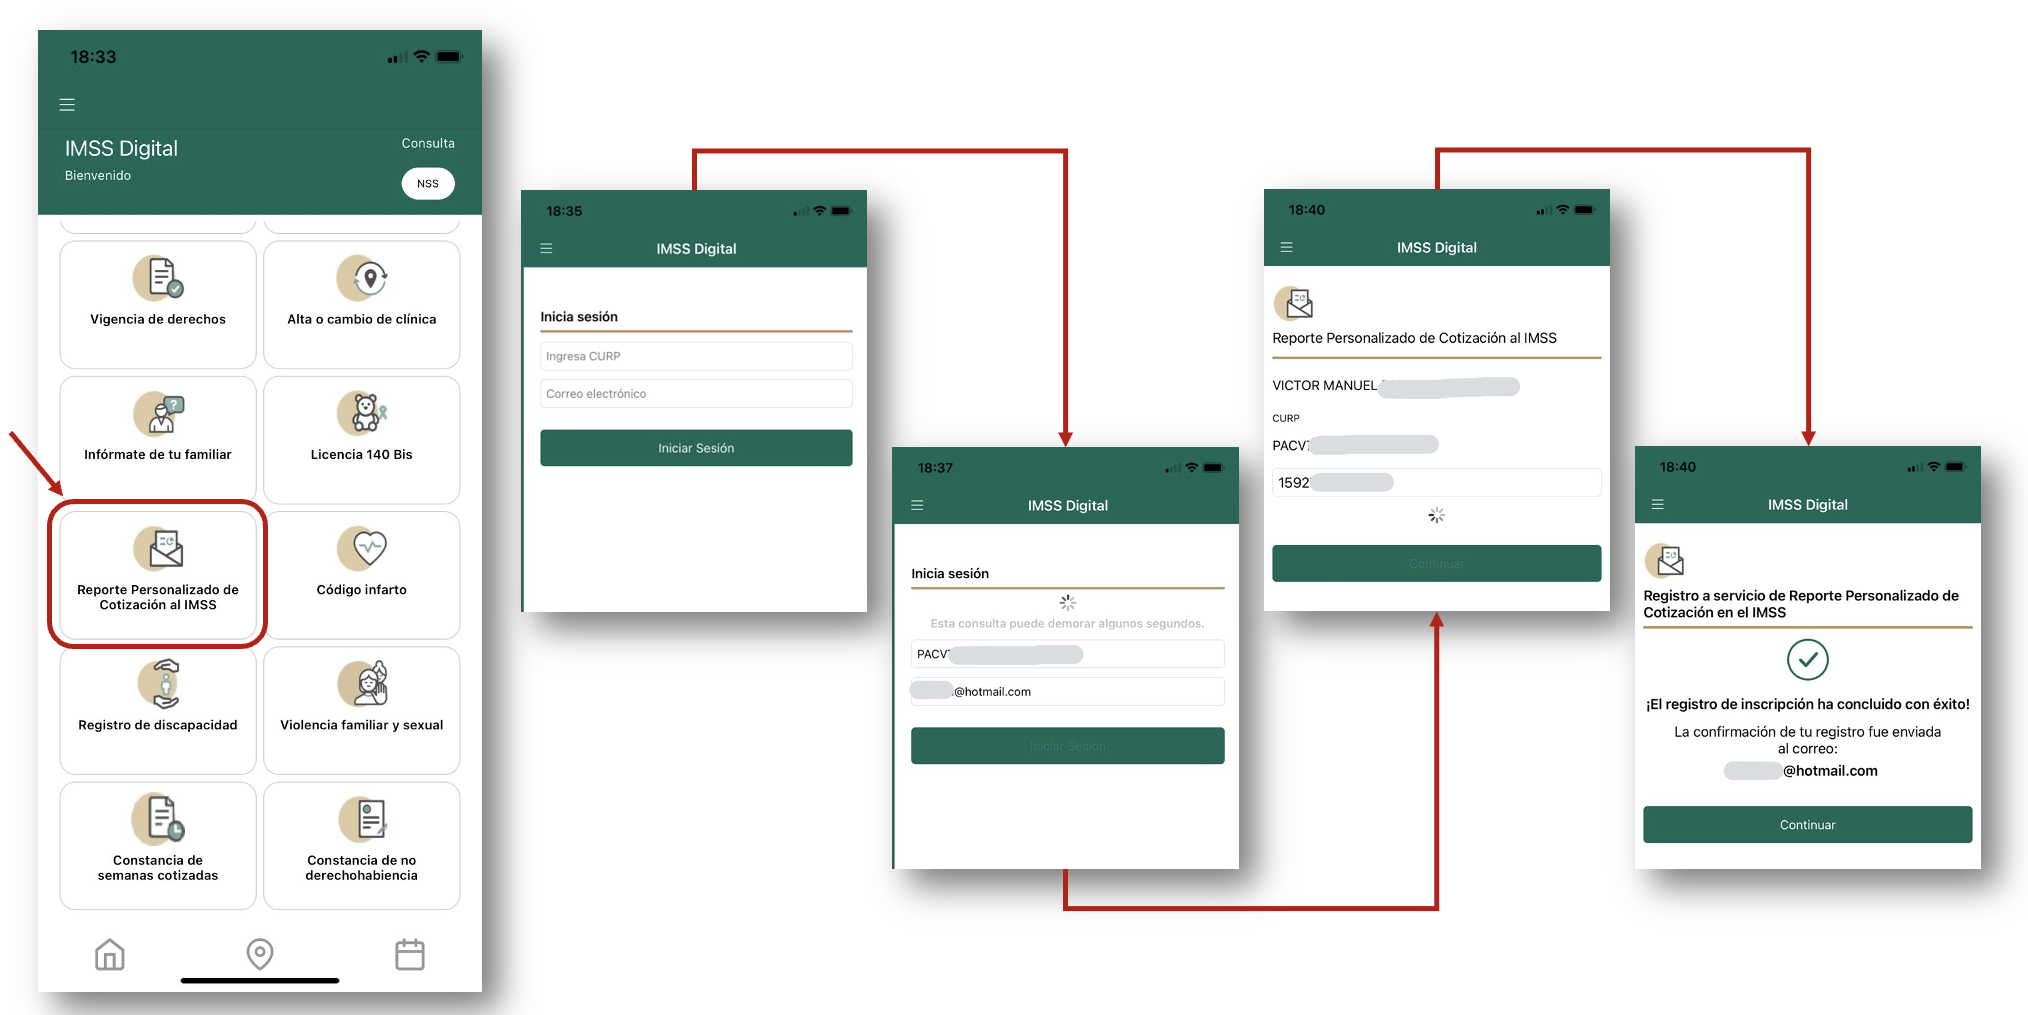
\includegraphics[width=\textwidth]{04_Figures/rpci_app/rpci_register.png}
    \end{subfigure}

    \end{center}
\end{figure}
\scriptsize{
\noindent Diagram shows how to register for the RPCI within the IMSS Digital app. The worker registers only once to access the RPCI, using his Unique Population Registry Key (CURP) and email address.
}

\clearpage

\begin{figure}[H]
    \caption{RPCI example}
    \label{rpci_example}
    \begin{center}
    
    \begin{subfigure}{0.49\textwidth}
    \caption{RPCI within the IMSS Digital app}
    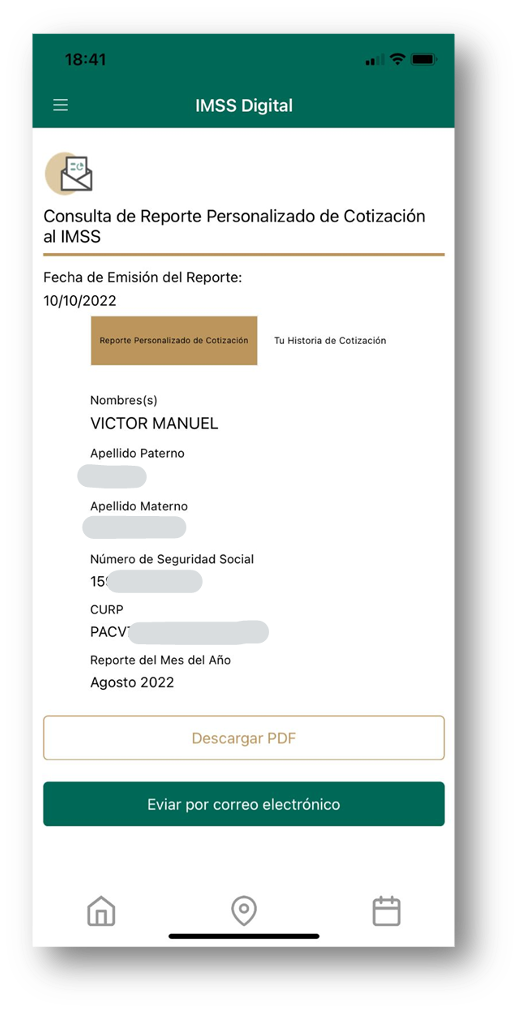
\includegraphics[width=\textwidth]{04_Figures/rpci_app/rpci_2.png}
    \end{subfigure}
    \begin{subfigure}{0.49\textwidth}
    \caption{RPCI PDF file}
    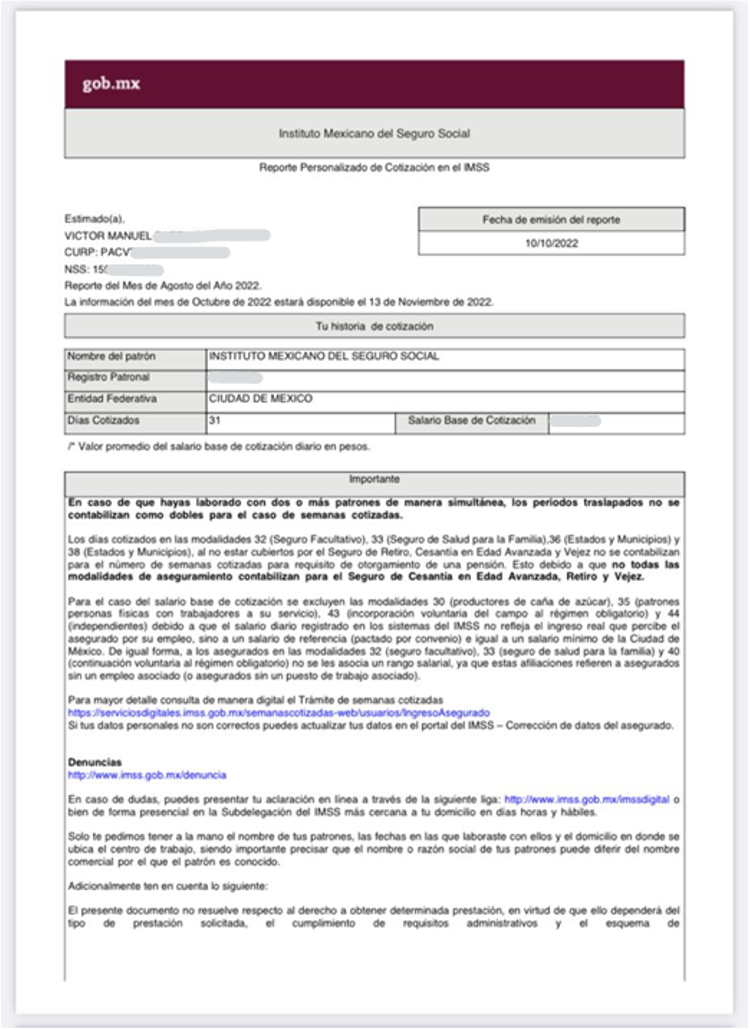
\includegraphics[width=\textwidth]{04_Figures/rpci_app/rpci_3.png}
    \end{subfigure}
    

    \end{center}
\end{figure}
\scriptsize{
\noindent Figure (a) shows the IMSS Digital app, where once the worker is registered for the RPCI, the worker can download their report in PDF or receive it via email. Figure (b) shows an example of the PDF for the RPCI. The report includes the worker job registered information, such as wage and the firm the worker is registered at.
}

%\clearpage

%\bibliographystyle{authordate1}
%\bibliographystyle{amsalpha}
%\bibliographystyle{AER}

%\bibliography{References}




% \end{document}

\end{document}

